\documentclass[fleqn]{NotesClass}

%% Packages
\usepackage{csquotes}
\usepackage{slashed}
\usepackage{subcaption}
\usepackage[version=4]{mhchem}

% ParticlesPackage
\usepackage{ParticlesPackage}
\makeatletter
\newcommand{\Pwboson}{\ensuremath{\PBASE@wboson}}
\newcommand{\PW}{\Pwboson}
\newcommand{\Pmuonneutral}{\ensuremath{\PBASE@muon}}
\newcommand{\Ptauneutral}{\ensuremath{\PBASE@tauon}}
\newcommand{\PJpsi}{\ensuremath{\mathrm{J}/\uppsi}}
\newcommand{\PBASE@pion}{\uppi}
\newcommand{\Ppi}{\ensuremath{\PBASE@pion}}
\newcommand{\Ppiplus}{\ensuremath{\PBASE@pion^+}}
\newcommand{\Ppiminus}{\ensuremath{\PBASE@pion^-}}
\newcommand{\Ppineutral}{\ensuremath{\PBASE@pion^0}}
\newcommand{\Ppip}{\Ppiplus}
\newcommand{\Ppim}{\Ppiminus}
\newcommand{\Ppizero}{\Ppineutral}
\newcommand{\PBASE@kaon}{\mathrm{K}}
\newcommand{\Pkaon}{\ensuremath{\PBASE@kaon}}
\newcommand{\PKshort}{\ensuremath{\PBASE@kaon_{\mathrm{S}}}}
\newcommand{\PKplus}{\ensuremath{\PBASE@kaon^+}}
\newcommand{\PKminus}{\ensuremath{\PBASE@kaon^-}}
\newcommand{\PKzero}{\ensuremath{\PBASE@kaon^0}}
\newcommand{\APKzero}{\ensuremath{\bar{\PBASE@kaon}}}
\newcommand{\PBASE@B}{\mathrm{B}}
\newcommand{\PB}{\ensuremath{\PBASE@B}}
\newcommand{\APB}{\ensuremath{\bar{\PBASE@B}}}
\newcommand{\Pfermion}{\ensuremath{\mathrm{f}}}
\newcommand{\APfermion}{\ensuremath{\bar{\mathrm{f}}}}
\newcommand{\Pphi}{\ensuremath{\upvarphi}}
\newcommand{\PBASE@Delta}{\Updelta}
\newcommand{\PDeltazero}{\ensuremath{\PBASE@Delta^0}}
\newcommand{\PDeltapp}{\ensuremath{\PBASE@Delta^{++}}}
\newcommand{\PDeltap}{\ensuremath{\PBASE@Delta^+}}
\newcommand{\PDeltam}{\ensuremath{\PBASE@Delta^-}}
\makeatother

% Tikz stuff
\usepackage{tikz}
\tikzset{>=latex}
% Externalise
\usetikzlibrary{external}
\tikzexternalize[prefix=tikz-external/]
% Other libraries
\usetikzlibrary{fadings}
\usetikzlibrary{decorations.pathreplacing}

% Tikz-Feynman
\usepackage[compat=1.1.0]{tikz-feynman}
\tikzfeynmanset{warn luatex=false}

% Siunitx
\usepackage{siunitx}
\DeclareSIUnit{\speedoflight}{\ensuremath{c}}
\DeclareSIUnit{\hbarunit}{\ensuremath{\hbar}}

% References, should be last things loaded
\usepackage{hyperref}  % Should be loaded second last (cleveref last)
\colorlet{hyperrefcolor}{blue!60!black}
\hypersetup{colorlinks=true, linkcolor=hyperrefcolor, urlcolor=hyperrefcolor}
\usepackage[
capitalize,
nameinlink,
noabbrev
]{cleveref} % Should be loaded last

% My packages
\usepackage{NotesBoxes}
\usepackage{NotesMaths}


% Title page info
\title{Relativity, Nuclear and Particle Physics\\{\Huge---Particle Physics}}
\author{Willoughby Seago}
\date{September 20, 2021}
% \subtitle{}
% \subsubtitle{}

% Highlight colour
%\definecolor{highlight}{HTML}{F36619}
\definecolor{darker}{HTML}{933808}
\definecolor{colder}{HTML}{863F86}
\definecolor{tetrad green}{HTML}{A8F31B}
\definecolor{tetrad blue}{HTML}{1BA8F3}
\definecolor{tetrad purple}{HTML}{671BF3}

% Commands
% math mode
\newcommand*{\baryonnumber}{\mathcal{B}}
\newcommand*{\luminosity}{\mathcal{L}}
\newcommand*{\e}{\mathrm{e}}
\newcommand*{\matrixelement}{\mathcal{M}}
\newcommand*{\branchingfraction}{\mathrm{BF}}
\newcommand*{\dalembertian}{\square^2}
\newcommand*{\ident}{I}
\newcommand*{\strong}{\mathrm{s}}
\newcommand*{\fermiconst}{G_{\mathrm{F}}}

% Include
\includeonly{}

\begin{document}
    \frontmatter
    \titlepage
    \title{Relativity, Nuclear and Particle Physics (Particle Physics)}
    \innertitlepage{} 
    \tableofcontents
    \listoftables
    \mainmatter
    
    \chapter{Introduction}
    In this course we introduce particle physics.
    The realm in which the physics of these particles lie is quantum field theory, although this is not the focus of this course.
    We will develop key ideas and along the way we will meet many particles.
    We will discus particle physics experiments and how we measure properties of particles.
    The focus will be on making sense of experimental observations without getting too bogged down in mathematical formalism.
    
    \part{The Basics}
    \chapter{The Standard Model}
    \section{What is Particle Physics?}
    Particle physics is about studying the fundamental constituents of matter, and some composite particles too.
    Such particles are small, and hence necessarily quantum mechanical, and travel fast, and hence necessarily relativistic.
    The realm in which quantum mechanics and relativity come together is quantum field theory (QFT)\glossary[acronym]{QFT}{quantum field theory}.
    While we won't fully develop QFT in this course we will use ideas from QFT as we see fit.
    
    The realm of particle physics is typically restricted to protons, neutrons, other similar composite particles, and fundamental particles.
    Once we get to a few nucleons we enter the range of nuclear physics, and if we start including electrons in this then we enter the range of atomic physics.
    
    As well as being interested in the building blocks of matter particle physics can also tell us about the initial state of the universe, after the big bang there was so much energy around that only particles could form for a very long time.
    Neutral atoms didn't form for millions of years after the big bang, so the early universe is the realm of nuclear and particle physics.
    
    \begin{figure}
        \tikzsetnextfilename{realms-of-physics}
        \begin{tikzpicture}
            \begin{scope}
                \clip (0, 0.5) rectangle (4.1, 2.6);
                \begin{scope}[transform canvas={rotate around={27.1:(2, 1.5)}}]
                    \fill[top color=highlight, bottom color=tetrad blue] (-0.25, -0.4) rectangle (4.4, 3.45);
                \end{scope}
            \end{scope}
            \node[white] at (1, 1) {\parbox{3cm}{\centering Quantum\\Mechanics}};
            \node[white] at (3, 1) {\parbox{3cm}{\centering Quantum\\Field Theory}};
            \node[white] at (1, 2) {\parbox{3cm}{\centering Classical\\Mechanics}};
            \node[white] at (3, 2) {\parbox{3cm}{\centering Special\\Relativity}};
            
            \draw[ultra thick, ->, tetrad blue] (0, 2.8) -- (4.1, 2.8) node[midway, black, above] {Speed};
            \draw[ultra thick, ->, tetrad blue] (-0.2, 2.6) -- (-0.2, 0.5) node[midway, black, left] {\rotatebox{90}{Size}};
            
            \draw[ultra thick, ->, path fading = west, tetrad blue] (0, 2.8) -- (4.1, 2.8);
            \draw[ultra thick, path fading = east, highlight] (0, 2.8) -- (4.1, 2.8);
            \draw[ultra thick, ->, path fading = north, tetrad blue] (-0.2, 2.6) -- (-0.2, 0.5);
            \draw[ultra thick, path fading = south, highlight] (-0.2, 2.6) -- (-0.2, 0.5);
        \end{tikzpicture}
        \caption{Realms of Physics.}
    \end{figure}
    
    \section{Natural Units}
    The SI\glossary[acronym]{SI}{le syst\`eme International d'Unit\`es} units that we are all familiar with are based on a set of base units, in particular length, in metres (\unit{\metre}), mass, in kilograms (\unit{\kilogram}), and time, in seconds (\unit{\second}).
    However, there is no particular reason why length, mass, and time should be our base units, and there is certainly no reason why we should measure them in kilograms, metres, and second.
    
    One simple alternative is the centimetre-gram-second system (CGS), where we still take length, mass, and time as the base units but now we measure length in centimetres (\unit{\centi\metre}), mass in grams (\unit{\gram}), and time in seconds (\unit{\second}).
    This system has some use, particularly in electromagnetism, but it's just a rescaling of the SI base units by a couple of factors of 1000, and isn't particularly suitable for particle physics.
    
    In particle physics we like to work with a system called \defineindex{natural units}.
    These typically give reasonable sized numbers in particle physics calculations.
    In this system the base units are energy, velocity, and action\footnote{\scriptsize \([\mathrm{velocity}] = [\mathrm{length}][\mathrm{time}]^{-1}\),\\\([\mathrm{energy}] = [\mathrm{mass}][\mathrm{length}]^2[\mathrm{time}]^{=2}\),\\\([\mathrm{action}] = [\mathrm{mass}][\mathrm{length}]^{2}[\mathrm{time}]^{-1}\)}.
    We measure energy in electronvolts (\unit{\electronvolt}), typically working with megaelectronvolts (\unit{\mega\electronvolt}), or gigaelectronvolts (\unit{\giga\electronvolt})\footnote{\(\qty{1}{\giga\electronvolt} = 10^3\,\unit{\mega\electronvolt} = 10^9\,\unit{\mathrm{\electronvolt}}\)}.
    We measure velocity in multiples of the speed of light (\unit{\speedoflight}).
    We measure action in multiples of the reduced Planck's constant (\unit{\hbarunit}).
    
    From these three base units we can define all other quantities of interest.
    In particular we can measure momentum in electronvolts per speed of light (\unit[per-mode=symbol]{\electronvolt\per\speedoflight}) and mass in electronvolts per speed of light squared (\unit[per-mode=symbol]{\electronvolt\per\speedoflight\squared}).
    We can check that this works out dimensionally by comparing to the SI base units:
    \begin{gather}
        [\mathrm{energy}][\mathrm{velocity}]^{-1} = \frac{[\mathrm{mass}][\mathrm{length}]^2[\mathrm{time}]^{-2}}{[\mathrm{length}] [\mathrm{time}]^{-1}}\\
        \qquad\qquad\qquad= [\mathrm{mass}][\mathrm{length}][\mathrm{time}]^{-1} = [\mathrm{momentum}]\\
        [\mathrm{energy}][\mathrm{velocity}]^{-2} = \frac{[\mathrm{mass}][\mathrm{length}]^2[\mathrm{time}]^{-2}}{([\mathrm{length}] [\mathrm{time}]^{-1})^2} = [\mathrm{mass}]
    \end{gather}
    Alternatively, we can check the units for consistency with \(E^2 = m^2c^4 + p^2c^2\), from which we get the same result if we measure \(E\) in electronvolts and take \(m\) or \(p\) to be zero.
    
    Other dimensions can also be expressed in electronvolts, speeds of light, and Planck's constants, in particular
    \begin{itemize}
        \item \([\mathrm{time}] = [\mathrm{action}] [\mathrm{energy}]^{-1}\), so time can be measured in \unit[per-mode=symbol]{\hbarunit\per\giga\electronvolt}.
        \item \([\mathrm{length}] = [\mathrm{action}] [\mathrm{velocity}] [\mathrm{energy}]^{-1}\), so length can be measured in \unit[per-mode=symbol]{\hbarunit\speedoflight\per\electronvolt}.
        \item \([\mathrm{area}] = [\mathrm{length}]^2\), so area can be measured in \unit[per-mode=symbol]{\hbarunit\squared\speedoflight\squared\per\giga\electronvolt\squared}.
    \end{itemize}
    
    So far we have only defined the relation between units, not the actual size of units.
    Of course, electronvolts, the speed of light, and Planck's constant all have well defined sizes, \emph{in SI units}, but we've come this far in abandoning SI units, it would be silly to cling to the values of a few constants now.
    Instead we usually choose the size of our units such that \(c = \hbar = 1\).
    In this case we don't write the factors of \(c\) and \(\hbar\) so we measure energy, mass, and momentum in \unit{\electronvolt}, time and length can be measured in \unit{\per\electronvolt}, and area in \unit{\per\electronvolt\squared}.
    
    One advantage of this system of units is that time and length are measured in the same units, which is good from a relativistic point of view as we should treat time and space in the same way.
    It also simplifies a lot of formulas in relativity and quantum mechanics by removing constants.
    For example
    \begin{gather}
        E^2 = m^2c^4 + p^2c^2 \to E^2 = m^2 + p^2,\\
        \left( \frac{\hbar^2}{2m}\laplacian - V(\vv{r})\right) \psi(\vv{r}, t) = i\hbar\diffp{\psi}{t} \to \left( \frac{1}{2m} \laplacian - V(\vv{r}) \right)\psi(\vv{r}, t) = i\diffp{\psi}{t},\\
        t = \frac{\tau}{\sqrt{1 + v^2/c^2}} \to t = \frac{\tau}{\sqrt{1 - v^2}}.
    \end{gather}
    
    To convert back to units where \(c, \hbar \ne 1\) we have to do some dimensional analysis, but generally the effort saved by setting \(c = \hbar = 1\) makes this extra work at the end worth while, if we always work in these units then the conversion work is minimised.
    
    \begin{exm}{}{}
        A \PW{} boson has energy width \(\Gamma = \qty{2}{\giga\electronvolt}\).
        What is the lifetime of the particle in SI units?
        The \defineindex{lifetime} of a particle is defined as \(\tau \coloneqq 1/\Gamma = \qty{0.5}{\giga\electronvolt}\)?
        
        Currently we have units of \([\mathrm{energy}]^{-1} = [\mathrm{E}]^{-1}\), and we need units of \([\mathrm{time}] = [\mathrm{T}]\).
        We get that by multiplying by some integer multiples of \(\hbar\) and \(c\), which have units of \([\hbar] = [\mathrm{E}][\mathrm{T}][\mathrm{L}]\), where \([\mathrm{L}] = [\mathrm{length}]\), and \([c] = [\mathrm{L}][\mathrm{T}]^{-1}\).
        Hence we need to find \(n, m \in \integers\) such that
        \begin{equation}
            [\mathrm{E}]^{-1}[\hbar]^{n}[c]^{m} = [\mathrm{T}].
        \end{equation}
        We will then have \(\tau = \hbar^nc^m/\Gamma\).
        We see that
        \begin{equation}
            [\mathrm{E}]^{-1}[\hbar]^{n}[c]^{m} = [\mathrm{E}]^{-1}[\mathrm{E}]^{n}[\mathrm{T}]^{n}[\mathrm{L}]^{m}[\mathrm{T}]^{-m}.
        \end{equation}
        From this w see that
        \(n = 1\) and \(m = 0\).
        Hence \(\tau = \hbar/\Gamma\), and so for the \PW{} boson \(\tau = \qty{0.5}{\hbar\per\giga\electronvolt}\).
    \end{exm}
    
    Natural units as defined here don't uniquely fix all dimensions.
    For example there are seven SI base units needed to fix all dimensions.
    We would need a similar number of base units in natural units also.
    Most of the time this isn't a problem as we aren't that interested in, say, the luminous intensity of a light source, so we don't need an equivalent to the candela (\unit{\candela}).
    Similarly we deal with a few particles at a time so don't need moles (\unit{\mole}).
    
    One quantity that we will need, which can't be expressed in natural units alone, is charge.
    In SI units the charge is fixed by defining the ampere as the rate of flow of charge.
    In particle physics we simply define charge as multiples of the electron charge, \(e\).
    Most fundamental particles have an integer multiple of \(e\) as their charge, with the exception of quarks, which have third integer multiples of \(e\).
    
    \section{Basic Particles}
    The \define{leptons}\index{lepton} are a family of particles made up of \define{electrons}\index{electron} (\Pe) and \define{electron neutrinos}\index{neutrino!electron}\index{electron!neutrino|see{neutrino, electron}} (\Pnue), as well as the heavier \defineindex{muon} (\Pmu) and \define{muon neutrino}\index{neutrino!muon}\index{muon!neutrino|see{neutrino, muon}} (\Pnumu), and the heavier still \defineindex{tau} (\Ptau) and \define{tau neutrino}\index{neutrino!tau}\index{tau!neutrino|see{neutrino, tau}} (\Pnutau).
    These are all \define{fermions}\index{fermion}, i.e. particles with half-integer spin, in particular leptons have spin\footnote{\(\hbar/2\) in non-natural units} \(1/2\).
    Electrons, muons, and tau have charge \(-e\).
    Neutrinos have no charge.
    The exact masses of the neutrinos aren't known, but it is known that they are very light, but have non-zero mass.
    We define three quantum numbers, the lepton family numbers, which correspond to electrons, muons, and tau.
    A lepton and the related neutrino have a lepton family number of \(+1\), and all other particles have 0.
    The properties of leptons are given in \cref{tab:lepton properties}.
    
    The \define{quarks}\index{quark} are a family of particles made up of up (\Pup), down (\Pdown), charm (\Pcharm), strange (\Pstrange), top (\Ptop), and bottom (\Pbottom) quarks.
    Of these three, \Pup, \Pcharm, \Ptop, have charge \(2e/3\), and the other three, \Pdown, \Pstrange, \Pbottom, have charge \(-e/3\).
    These are also fermions with spin \(1/2\).
    The properties of quarks are given in \cref{tab:quark properties}.
    
    As well as the leptons and quarks there are the antileptons and antiquarks.
    These have the same mass but their charges and additive quantum numbers are negated.
    For example, antielectrons, also known as \define{positrons}\index{positron} (\APe) have electron lepton family member \(L_{\Pelectronneutral} = -1\), antiquarks have baryon number \(-1/3\), and antistrange quarks have strangeness quantum number \(+1\).
    For particles with an explicit charge, such as \(\Ptau\), we denote the antiparticle by negating the charge, so \(\APtau\).
    For particles without an explicit charge, for example, \(\Pup\), we denote the antiparticle with a bar, so \(\APup\).
    
    \begin{table}
        \caption[Lepton properties]{Some key properties of leptons, including the generation, charge, mass, and lepton flavour number, specifically the electron, muon, and tau lepton family numbers, \(L_{\Pelectronneutral}\), \(L_{\Pmuonneutral}\), and \(L_{\Ptauneutral}\) respectively.}
        \label{tab:lepton properties}
        \begin{tabular}{cccccccc}\toprule
            Lepton & \rotatebox{67}{\hspace{-1.5em}Symbol} & \rotatebox{67}{\hspace{-1.5em}Generation} & \rotatebox{67}{\hspace{-1.5em}Charge/\(e\)} & \rotatebox{67}{\hspace{-1.5em}Mass/\unit{\mega\electronvolt}} & \multicolumn{3}{c}{Lepton Family Number}\\
            &&&&& \(L_{\Pelectronneutral}\) & \(L_{\Pmuonneutral}\) & \(L_{\Ptauneutral}\) \\\midrule
            Electron & \Pe & 1 & -1 & \(0.511\) & 1 & 0 & 0\\
            Electron Neutrino & \Pnue & 1 & 0 & \(<\num{2.1e-6}\) & 1 & 0 & 0\\\midrule
            Muon & \Pmuon & 2 & -1 & \(105.66\) & 0 & 1 & 0\\
            Muon Neutrino & \Pnumu & 2 & 0 & \(<0.19\) & 0 & 1 & 0\\\midrule
            Tau & \Ptau & 3 & -1 & \(1777\) & 0 & 0 & 1\\
            Tau Neutrino & \Pnutau & 3 & 0 & \(<18\) & 0 & 0 & 1\\\bottomrule
        \end{tabular}
    \end{table}
    
    \begin{table}
        \caption[Quark properties.]{Some key properties of quarks, including the generation, charge, mass, isospin, quark flavour number, and baryon number.}
        \label{tab:quark properties}
        \begin{tabular}{cccccccc}\toprule
            Quark & \rotatebox{78}{Symbol} & \rotatebox{78}{Generation} & \rotatebox{78}{Charge/\(e\)} & \rotatebox{78}{Mass/\unit{\mega\electronvolt}} & \rotatebox{78}{Isospin \((I, I_z)\)} & \rotatebox{78}{\hspace{-0.7em}\parbox{3cm}{\centering Quark Flavour Quantum Number}\hspace{-0.8em}} & \rotatebox{78}{\parbox{2cm}{\centering Baryon Number, \(\baryonnumber\)}}\\\midrule
            Up      & \Pup      & 1 & \(2/3\)  & \(2.2\)  & \((1/2, +1/2)\) &            & \(1/3\) \\
            Down    & \Pdown    & 1 & \(-1/3\) & \(4.7\)  & \((1/2, -1/2)\) &            & \(1/3\) \\
            Charm   & \Pcharm   & 2 & \(2/3\)  & \(1270\) &                 & \(C = +1\) & \(1/3\) \\
            Strange & \Pstrange & 2 & \(-1/3\) & \(93\)   &                 & \(S = -1\) & \(1/3\) \\
            Top     & \Ptop     & 3 & \(2/3\)  & \(\num{172.9e3}\) &                 & \(T = +1\) & \(1/3\) \\
            Bottom  & \Pbottom  & 3 & \(-1/3\) & \(4180\) &                 & \(B = -1\) & \(1/3\) \\\bottomrule
        \end{tabular}
    \end{table}
    
    \subsection{A Brief History of Particle Discoveries}
    \begin{enumerate}
        \item[1887] The electron was discovered by J.~J.~Thompson.
        \item[1920] The proton was discovered by E.~Rutherford.
        \item[1931] The positron was discovered by C.~Anderson.
        It was originally thought to be a proton.
        \item[1936] The muon was discovered by C.~Anderson\footnote{leave some for everyone else Anderson.}.
        \item[1956] The electron neutrino was discovered by C.~Cowan and F.~Reines.
        \item[1962] The muon neutrino was discovered by L.~Lederman, M.~Schwartz, and J.~Steinberger.
        \item[1968] It was discovered that the proton is made of quarks, in particular the proton is \Pu\Pu\Pd, this was discovered by J.~Friedman \textit{et al.} at the Stanford linear accelerator centre (SLAC)\glossary[acronym]{SLAC}{Stanford linear accelerator laboratory}.
        \item[1973] The \PJpsi{} resonance was discovered, which is the most common resonance of charmonium, a charm-anticharm quark meson (\Pc\APc).
        This was evidence for the charm quark, and was discovered by B.~Richter \textit{et al.} SLAC as well as the Brookhaven national laboratory (BNL)\glossary[acronym]{BNL}{Brookhaven national laboratory}.
        \item[1975] The tau was discovered by M.~Perl \textit{et al.} at SLAC.
        \item[1977] The \(\upUpsilon\) resonance was discovered, which is a resonance of bottomonium, a bottom-antibottom quark meson (\Pb\APb).
        This was evidence for the bottom quark, and was discovered by L.~Lederman\footnote{another greedy particle physicist, discovering all the particles for himself.} \textit{et al.} at Fermilab.
        \item[1995] The top quark was discovered by the collider detector at Fermilab (CDF)\glossary[acronym]{CDF}{collider detector at Fermilab} and the DØ experiment (DZero experiment) also at Fermilab.
        \item[2000] The tau neutrino was discovered by the direct observation of the nu tau experiment, or the DONUT\glossary[acronym]{DONUT}{direct observation of the nu tau}\footnote{they really \emph{really} wanted that acronym to work.} experiment.
        \item[2021] The Higgs was discovered in 2012 by a toroidal LHC apparatus (ATLAS)\footnote{surely the acronym with the word \enquote{toroidal} should be the one to spell DONUT} and the compact muon solenoid (CMS)\glossary[acronym]{CMS}{compact muon solenoid} experiments at \textit{conseil europ\'een pour la recherche nucl\'eaire} (CERN)\glossary[acronym]{CERN}{\textit{conseil europ\'een pour la recherche nucl\'eaire}}, with the large hadron collider (LHC)\glossary[acronym]{LHC}{large hadron collider}.
    \end{enumerate}

    \subsection{Fundamental Forces}
    There are four fundamental forces:
    \begin{itemize}
        \item The strong force
        \item Electromagnetism
        \item The weak force
        \item Gravity
    \end{itemize}
    Of these only the first three are important at the subatomic level.
    For example, the strong force binds quarks into nucleons, electromagnetism governs the interaction of electrons, and the weak force controls the decay of radioactive nuclei.
    Gravity is simply too weak to have any noticeable effect on these scales.
    
    The fundamental forces are propagated by \defineindex{messenger particles}, all of which are \define{bosons}, i.e. particles with integer spin.
    In particular they are \define{vector bosons}\index{boson!vector}, meaning they have spin 1.
    For example the \PWm{} boson is the exchange boson in beta decay of a neutron, \(\Pn \to \Pp \Pe \APnue\).
    Information on the fundamental forces and their exchange bosons is given in
    
    \begin{table}
        \caption[Vector boson information]{Information on the messenger particles for the four fundamental forces. Note that the existence of the graviton has not been experimentally verified.}
        \begin{tabular}{cccc}\toprule
            Force & Boson & Mass/\unit{\giga\electronvolt} & Relative Strength\\\midrule
            Strong & Gluon & 0 & 1\\
            EM & Photon & 0 & \num{e-2}\\
            Weak & \Pwboson/\PZ & \(80.4\), \(91.2\) & \num{e-7}\\
            Gravity & Graviton (???) & 0 & \num{e-40}\\\bottomrule
        \end{tabular}
    \end{table}
    
    \section{Space-Time Symmetries}
    \begin{thm}{Noether's Theorem}{}
        Every continuous symmetry of nature corresponds to a conservation law.
    \end{thm}
    Noether's theorem relates continuous symmetries (in particular symmetries under which the Lagrangian is invariant) to conservation laws.
    The three most common examples being
    \begin{itemize}
        \item Invariance under spatial translation giving momentum conservation.
        \item Invariance under time translation giving conservation of energy.
        \item Invariance under rotation giving conservation of angular momentum.
    \end{itemize}
    Notice that in relativity the first two become one and invariance under translations of the four-position lead to conservation of the four-momentum.
    
    Noether's theorem deals with continuous symmetries, in the sense that we can consider arbitrarily small translations or rotations.
    There are also symmetries relating to discrete symmetries, and these too lead to conservation laws.
    There are other conservation laws that we have observed but do not know what symmetry leads to them, if indeed there is a symmetry at all.
    
    These conservation laws are usually phrased in terms of conservation of quantum numbers.
    Many of these are familiar already.
    
    The \defineindex{charge} is a quantum number, which measures the strength of interactions with the electromagnetic field.
    
    The \defineindex{lepton flavour number} is a quantum number, in particular we define the electron lepton flavour number as
    \begin{equation}
        L_{\Pelectronneutral} \coloneqq N(\Pe) + N(\Pnue) - N(\APe) - N(\APnue).
    \end{equation}
    Here \(N(x)\) is the number of \(x\) present in the system.
    We define the muon and tau lepton flavour numbers analogously.
    The \defineindex{lepton number} is then simply the sum of these,
    \begin{equation}
        L \coloneqq L_{\Pelectronneutral} + L_{\Pmuonneutral} + L_{\Ptauneutral}.
    \end{equation}
    Which is just the number of leptons minus the number of antileptons.
    
    The \defineindex{quark flavour number} is a quantum number, for up quarks we define it as
    \begin{equation}
        N_{\Pu} \coloneq N(u) - N(\APu).
    \end{equation}
    We define analogous quantities for the other quark flavours.
    The \defineindex{quark number} is simply the total number of quarks minus the number of antiquarks,
    \begin{equation}
        N_{\Pq} \coloneqq N(\Pq) - N(\APq) = N_{\Pu} + N_{\Pd} + N_{\Pc} + N_{\Ps}+ N_{\Pt} + N_{\Pb}.
    \end{equation}
    
    The \defineindex{baryon number} is three times the quark number, that is
    \begin{equation}
        \baryonnumber \coloneqq 3N_{\Pq} = 3(N_{\Pu} + N_{\Pd} + N_{\Pc} + N_{\Ps}+ N_{\Pt} + N_{\Pb}).
    \end{equation}
    Notice that by this definition quarks all have a baryon number of \(1/3\), and antiquarks have \(-1/3\).
    
    \begin{itemize}
        \item Invariance under gauge transformation\footnote{a gauge transformation in this case acting on the electromagnetic potentials is the transformation \(\varphi \to \varphi - \partial_t\chi\) and \(\vv{A} \to \vv{A} + \grad\chi\), for scalar and vector potentials \(\varphi\) and \(\vv{A}\) and some arbitrary, twice differentiable, function of space and time, \(\chi\). Relativistically this is the same as \(A_\mu \to A_\mu - \partial_\mu\) where \(A^\mu = (\varphi, \vv{A})\) is the four-potential and \(\partial_\mu = (\partial_t, \grad)\).} in quantum electrodynamics (QED)\glossary[acronym]{QED}{quantum electrodynamics} leads to charge conservation.
        \item The lepton flavour numbers, \(L_{\Pelectronneutral}\), \(L_{\Pmuonneutral}\), and \(L_{\Ptauneutral}\), are conserved in all known interactions, and hence the lepton number, \(L\), is conserved.
        There is no known symmetry leading to this.
        \item The quark flavour numbers, \(N_{\Pu}\), \(N_{\Pd}\), \(N_{\Pc}\), \(N_{\Ps}\), \(N_{\Pt}\), and \(N_{\Pb}\), and hence the quark number, \(N_{\Pq}\), and baryon number, \(\baryonnumber\), are conserved in quantum chromodynamics (QCD)\glossary[acronym]{QCD}{quantum chromodynamics}, and QED, but not in weak interactions.
        There is no known symmetry leading to this.
        \item Parity\footnote{Recall that the parity of a state, \(\psi\), is the eigenvalue of the operation \(\psi(\vv{r}) \to \psi(-\vv{r})\), in particular if \(\psi(-\vv{r}) = \pm \psi(\vv{r})\) we say that the parity is even (\(+\)) or odd (\(-\)).} is conserved in QCD and QED, but not in weak interactions.
        There is no known symmetry leading to this.
    \end{itemize}
    
    \section{Open Questions}
    There are many open questions in particle theory.
    For example, the unknown symmetries mentioned in the previous section.
    Other questions include
    \begin{itemize}
        \item There are three generations of quarks and leptons.
        Why?
        Why not 2 or 3, why do we even \enquote{need} more than 1?
        \item The mass difference between generations is large.
        Why?
        \item What about the stuff not in the standard model?
        What is dark matter/dark energy and how does it fit with the standard model?
    \end{itemize}
    This last question is fairly large given that approximately \qty{95}{\percent} of the universe is dark matter or dark energy.
    
    \begin{figure}
        \tikzsetnextfilename{standard-model}
        \begin{tikzpicture}
            \tikzset{box/.style = {rounded corners, ultra thick, color=#1}}
            % Gen 1
            % electron neutrino
            \draw[box=highlight, fill=highlight!50] (0, 0) rectangle (2, 2);
            \node[font=\sffamily\tiny] at (1, 0.2) {Electron Neutrino};
            \node[font=\Huge] at (1, 1) {\(\upnu_\mathsf{e}\)};
            \node[font=\sffamily\tiny, right] at (0, 1.8) {\(<\qty{2.2}{\electronvolt}\)};
            \node[font=\sffamily\tiny, right] at (0, 1.5) {\(0\)};
            \node[font=\sffamily\tiny, right] at (0, 1.2) {\(1/2\)};
            % electron
            \begin{scope}[yshift=2.2cm]
                \draw[box=highlight, fill=highlight!50] (0, 0) rectangle (2, 2);
                \node[font=\sffamily\tiny] at (1, 0.2) {Electron};
                \node[font=\Huge] at (1, 1) {\(\mathsf{e}\)};
                \node[font=\sffamily\tiny, right] at (0, 1.8) {\(\qty{511}{\kilo\electronvolt}\)};
                \node[font=\sffamily\tiny, right] at (0, 1.5) {\(-1\)};
                \node[font=\sffamily\tiny, right] at (0, 1.2) {\(1/2\)};
            \end{scope}
            % down
            \begin{scope}[yshift=4.4cm]
                \draw[box=tetrad purple, fill=tetrad purple!50] (0, 0) rectangle (2, 2);
                \node[font=\sffamily\tiny] at (1, 0.2) {Down};
                \node[font=\Huge] at (1, 1) {\(\mathsf{d}\)};
                \node[font=\sffamily\tiny, right] at (0, 1.8) {\(\approx\qty{4.8}{\mega\electronvolt}\)};
                \node[font=\sffamily\tiny, right] at (0, 1.5) {\(-1/3\)};
                \node[font=\sffamily\tiny, right] at (0, 1.2) {\(1/2\)};
            \end{scope}
            % up
            \begin{scope}[yshift=6.6cm]
                \draw[box=tetrad purple, fill=tetrad purple!50] (0, 0) rectangle (2, 2);
                \node[font=\sffamily\tiny] at (1, 0.2) {Up};
                \node[font=\Huge] at (1, 1) {\(\mathsf{u}\)};
                \node[font=\sffamily\tiny, right] at (0, 1.8) {\(\approx\qty{2.3}{\mega\electronvolt}\)};
                \node[font=\sffamily\tiny, right] at (0, 1.5) {\(2/3\)};
                \node[font=\sffamily\tiny, right] at (0, 1.2) {\(1/2\)};
            \end{scope}
            % Gen 2
            \begin{scope}[xshift=2.2cm]
                % muon neutrino
                \draw[box=highlight!80, fill=highlight!30] (0, 0) rectangle (2, 2);
                \node[font=\sffamily\tiny] at (1, 0.2) {upmuon Neutrino};
                \node[font=\Huge] at (1, 1) {\(\upnu_\upmu\)};
                \node[font=\sffamily\tiny, right] at (0, 1.8) {\(<\qty{0.17}{\mega\electronvolt}\)};
                \node[font=\sffamily\tiny, right] at (0, 1.5) {\(0\)};
                \node[font=\sffamily\tiny, right] at (0, 1.2) {\(1/2\)};
                % muon
                \begin{scope}[yshift=2.2cm]
                    \draw[box=highlight, fill=highlight!30] (0, 0) rectangle (2, 2);
                    \node[font=\sffamily\tiny] at (1, 0.2) {upmuon};
                    \node[font=\Huge] at (1, 1) {\(\upmu\)};
                    \node[font=\sffamily\tiny, right] at (0, 1.8) {\(\qty{105.7}{\mega\electronvolt}\)};
                    \node[font=\sffamily\tiny, right] at (0, 1.5) {\(-1\)};
                    \node[font=\sffamily\tiny, right] at (0, 1.2) {\(1/2\)};
                \end{scope}
                % strange
                \begin{scope}[yshift=4.4cm]
                    \draw[box=tetrad purple!80, fill=tetrad purple!30] (0, 0) rectangle (2, 2);
                    \node[font=\sffamily\tiny] at (1, 0.2) {Down};
                    \node[font=\Huge] at (1, 1) {\(\mathsf{s}\)};
                    \node[font=\sffamily\tiny, right] at (0, 1.8) {\(\approx\qty{1.275}{\giga\electronvolt}\)};
                    \node[font=\sffamily\tiny, right] at (0, 1.5) {\(-1/3\)};
                    \node[font=\sffamily\tiny, right] at (0, 1.2) {\(1/2\)};
                \end{scope}
                % charm
                \begin{scope}[yshift=6.6cm]
                    \draw[box=tetrad purple!80, fill=tetrad purple!30] (0, 0) rectangle (2, 2);
                    \node[font=\sffamily\tiny] at (1, 0.2) {Charm};
                    \node[font=\Huge] at (1, 1) {\(\mathsf{c}\)};
                    \node[font=\sffamily\tiny, right] at (0, 1.8) {\(\approx\qty{95}{\mega\electronvolt}\)};
                    \node[font=\sffamily\tiny, right] at (0, 1.5) {\(2/3\)};
                    \node[font=\sffamily\tiny, right] at (0, 1.2) {\(1/2\)};
                \end{scope}
            \end{scope}
            % Gen 3
            \begin{scope}[xshift=4.4cm]
                % tau neutrino
                \draw[box=highlight!60, fill=highlight!10] (0, 0) rectangle (2, 2);
                \node[font=\sffamily\tiny] at (1, 0.2) {uptau Neutrino};
                \node[font=\Huge] at (1, 1) {\(\upnu_\uptau\)};
                \node[font=\sffamily\tiny, right] at (0, 1.8) {\(<\qty{15.5}{\mega\electronvolt}\)};
                \node[font=\sffamily\tiny, right] at (0, 1.5) {\(0\)};
                \node[font=\sffamily\tiny, right] at (0, 1.2) {\(1/2\)};
                % tau
                \begin{scope}[yshift=2.2cm]
                    \draw[box=highlight!60, fill=highlight!10] (0, 0) rectangle (2, 2);
                    \node[font=\sffamily\tiny] at (1, 0.2) {uptau};
                    \node[font=\Huge] at (1, 1) {\(\uptau\)};
                    \node[font=\sffamily\tiny, right] at (0, 1.8) {\(\qty{1.777}{\giga\electronvolt}\)};
                    \node[font=\sffamily\tiny, right] at (0, 1.5) {\(-1\)};
                    \node[font=\sffamily\tiny, right] at (0, 1.2) {\(1/2\)};
                \end{scope}
                % bottom
                \begin{scope}[yshift=4.4cm]
                    \draw[box=tetrad purple!60, fill=tetrad purple!10] (0, 0) rectangle (2, 2);
                    \node[font=\sffamily\tiny] at (1, 0.2) {Bottom};
                    \node[font=\Huge] at (1, 1) {\(\mathsf{b}\)};
                    \node[font=\sffamily\tiny, right] at (0, 1.8) {\(\approx\qty{4.18}{\giga\electronvolt}\)};
                    \node[font=\sffamily\tiny, right] at (0, 1.5) {\(-1/3\)};
                    \node[font=\sffamily\tiny, right] at (0, 1.2) {\(1/2\)};
                \end{scope}
                % up
                \begin{scope}[yshift=6.6cm]
                    \draw[box=tetrad purple!60, fill=tetrad purple!10] (0, 0) rectangle (2, 2);
                    \node[font=\sffamily\tiny] at (1, 0.2) {Top};
                    \node[font=\Huge] at (1, 1) {\(\mathsf{t}\)};
                    \node[font=\sffamily\tiny, right] at (0, 1.8) {\(\approx\qty{173.07}{\giga\electronvolt}\)};
                    \node[font=\sffamily\tiny, right] at (0, 1.5) {\(2/3\)};
                    \node[font=\sffamily\tiny, right] at (0, 1.2) {\(1/2\)};
                \end{scope}
            \end{scope}
            % Vector bosons
            \begin{scope}[xshift=6.6cm]
                % gluon
                \draw[box=tetrad green, fill=tetrad green!50] (0, 0) rectangle (2, 2);
                \node[font=\sffamily\tiny] at (1, 0.2) {Gluon};
                \node[font=\Huge] at (1, 1) {\(\mathsf{g}\)};
                \node[font=\sffamily\tiny, right] at (0, 1.8) {\(0\)};
                \node[font=\sffamily\tiny, right] at (0, 1.5) {\(0\)};
                \node[font=\sffamily\tiny, right] at (0, 1.2) {\(1\)};
                % photon
                \begin{scope}[yshift=2.2cm]
                    \draw[box=tetrad green, fill=tetrad green!50] (0, 0) rectangle (2, 2);
                    \node[font=\sffamily\tiny] at (1, 0.2) {Photon};
                    \node[font=\Huge] at (1, 1) {\(\upgamma\)};
                    \node[font=\sffamily\tiny, right] at (0, 1.8) {\(0\)};
                    \node[font=\sffamily\tiny, right] at (0, 1.5) {\(0\)};
                    \node[font=\sffamily\tiny, right] at (0, 1.2) {\(1\)};
                \end{scope}
                % Z
                \begin{scope}[yshift=4.4cm]
                    \draw[box=tetrad green, fill=tetrad green!50] (0, 0) rectangle (2, 2);
                    \node[font=\sffamily\tiny] at (1, 0.2) {Z Boson};
                    \node[font=\Huge] at (1, 1) {\(\mathsf{Z}\)};
                    \node[font=\sffamily\tiny, right] at (0, 1.8) {\(\qty{91.2}{\giga\electronvolt}\)};
                    \node[font=\sffamily\tiny, right] at (0, 1.5) {\(0\)};
                    \node[font=\sffamily\tiny, right] at (0, 1.2) {\(1\)};
                \end{scope}
                % W
                \begin{scope}[yshift=6.6cm]
                    \draw[box=tetrad green, fill=tetrad green!50] (0, 0) rectangle (2, 2);
                    \node[font=\sffamily\tiny] at (1, 0.2) {W Boson};
                    \node[font=\Huge] at (1, 1) {\(\mathsf{W}\)};
                    \node[font=\sffamily\tiny, right] at (0, 1.8) {\(\qty{80.4}{\giga\electronvolt}\)};
                    \node[font=\sffamily\tiny, right] at (0, 1.5) {\(\pm 1\)};
                    \node[font=\sffamily\tiny, right] at (0, 1.2) {\(1\)};
                \end{scope}
            \end{scope}
            % Higgs
            \begin{scope}[xshift=8.8cm, yshift=6.6cm]
                \draw[box=tetrad blue, fill=tetrad blue!50] (0, 0) rectangle (2, 2);
                \node[font=\sffamily\tiny] at (1, 0.2) {Higgs Boson};
                \node[font=\Huge] at (1, 1) {\(\mathsf{H}\)};
                \node[font=\sffamily\tiny, right] at (0, 1.8) {\(\qty{125}{\giga\electronvolt}\)};
                \node[font=\sffamily\tiny, right] at (0, 1.5) {\(0\)};
                \node[font=\sffamily\tiny, right] at (0, 1.2) {\(0\)};
            \end{scope}
            \node[font=\sffamily\bfseries\huge, tetrad purple] at (-0.35, 6.6) {\rotatebox{90}{Quarks}};
            \node[font=\sffamily\bfseries\huge, highlight] at (-0.35, 2.2) {\rotatebox{90}{Leptons}};
            \node[font=\sffamily\bfseries\huge, tetrad green] at (9.05, 3.3) {\rotatebox{90}{Vector Bosons}};
            \node[font=\sffamily\bfseries\huge, tetrad blue] at (9.6, 3.3) {\rotatebox{-90}{Scalar Bosons}};
            
            \begin{scope}[yshift=6.6cm]
                \node[left, font=\sffamily\tiny] at (0, 1.8) {Mass};
                \node[left, font=\sffamily\tiny] at (0, 1.5) {Charge};
                \node[left, font=\sffamily\tiny] at (0, 1.2) {Spin};
            \end{scope}
        \end{tikzpicture}
        \caption[The standard model.]{Particles of the standard model, with their masses, charges, spins, symbols, and names.}
    \end{figure}
    
    \chapter{Tools of Particle Physics}
    \section{Measurable Properties}
    There are many properties of particles that we may wish to measure.
    These broadly separate into two categories, static properties, which don't change, and dynamic properties which do.
    Examples of static properties includes
    \begin{itemize}
        \item Mass, \(m\).
        \item Charge, \(Q\).
        \item Spin, \(J\), and parity, \(P\), together \(J^P\).
        \item Colour charge (see \cref{sec:colour}).
        \item Weak hypercharge (see ). % TODO: add reference to section where weak hypercharge is introduced
    \end{itemize}
    Examples of dynamic properties includes
    \begin{itemize}
        \item Energy, \(E\).
        \item Momentum, \(p\).
    \end{itemize}
    
    There are typically two ways that we measure properties.
    We need some sort of interaction in order to extract information from the system, the common interactions used are particle decay and particle scattering.
    Particle decays can tell us
    \begin{itemize}
        \item Particle lifetime, \(\tau\).
        \item Decay width, \(\Gamma = \hbar / \tau\).
        \item Allowed and forbidden decays, which imply conservation laws.
    \end{itemize}
    Particle scattering can tell us
    \begin{itemize}
        \item Total cross section, \(\sigma\).
        \item Differential cross section, \(\diff{\sigma}/{\Omega}\).
        \item Luminosity, \(\luminosity\) (see \cref{sec:particle scattering}).
        \item Event rate, \(N\).
    \end{itemize}
    
    \section{Relativity Recap}
    \begin{rmk}
        See the notes for the relativity part of the course for more details.
    \end{rmk}
    Recall that we define \(\beta \coloneqq v/c\).
    In natural units \(\beta = v\) and we use them interchangeably.
    The Lorentz gamma factor is then
    \begin{equation}
        \gamma \coloneqq \frac{1}{\sqrt{1 - \beta^2}}.
    \end{equation}
    The relativistic three-momentum of the particle is defined as \(\vv{p} \coloneqq \gamma m\vv{v}\).
    The relativistic energy of a particle is defined as
    \begin{equation}
        E^2 = m^2c^4 + p^2c^2
    \end{equation}
    where \(p = \abs{\vv{p}}\).
    The energy is also given by \(E = \gamma mc^2\).
    In natural units these equations reduce to
    \begin{equation}
        E^2 = m^2 + p^2, \qqand E = \gamma m.
    \end{equation}
    We also have \(\beta = \abs{\vv{p}}/E\) and so \(\beta\gamma = \abs{\vv{p}}/m\).
    The four-momentum of the particle is then \(p^\mu = (E/c, \vv{p})\), or in natural units \(p^\mu = (E, \vv{p})\).
    
    For a massless particle \(v = c\), \(\beta = 1\), and \(E = p\), the gamma factor, \(\gamma\), is not defined.
    
    For a particle at rest \(v = \beta = 0\), \(E = m\), and \(\gamma = 1\).
    
    The invariant mass of a particle is defined as the square of its four momentum,
    \begin{equation}
        p^2 = p_\mu p^\mu = E^2 - \vv{p}^2 = m^2
    \end{equation}
    where the final equality comes from evaluating the scalar product, which is a Lorentz invariant, in the rest frame of the particle.
    
    \section{Quantum Mechanics Recap}
    A free particle in three dimensional space has a wave function given by
    \begin{equation}
        \psi(\vv{r}, t) = \exp[i(\vv{p} \cdot \vv{r} - Et)/\hbar]
    \end{equation}
    where \(\vv{r}\) is the position of the particle, \(\vv{p}\) is the momentum of the particle, \(E\) is the energy of the particle, and \(t\) is the time.
    
    Define the momentum operator, \(\vecoperator{p} = -i\hbar\grad\), and energy operator, \(\operator{E} \coloneqq i\hbar\partial_t\).
    Using the non-relativistic kinetic energy, \(E = p^2/(2m)\), as the energy of the particle replacing \(E\) and \(p\) with their operators we get
    \begin{equation}
        i\hbar \diffp{\psi}{t} = -\frac{\hbar^2}{2m}\laplacian\psi
    \end{equation}
    which is the Schr\"odinger equation.
    In natural units this reduces to
    \begin{equation}
        i\diffp{\psi}{t} = -\frac{1}{2n}\laplacian\psi.
    \end{equation}
    The Schr\"odinger equation is non-relativistic, since we used \(E = p^2/(2m)\), and it is not Lorentz invariant.
    
    \section{Relativistic Quantum Mechanics}\label{sec:relativistic quantum mechanics}
    \begin{rmk}
        See Quantum Theory notes for more detail.
    \end{rmk}
    If we instead use the full relativistic energy, \(E^2 = m^2c^4 + p^2c^2\) we get the equation
    \begin{equation}
        -\hbar^2\diffp[2]{\psi}{t} = -\hbar^2c^2\laplacian\psi + m^2c^4\psi.
    \end{equation}
    This is the \defineindex{Klein--Gordan} equation, which can be written in natural units as
    \begin{equation}
        -\diffp[2]{\psi}{t} = -\laplacian\psi + m^2\psi.
    \end{equation}
    
    Notice that the relativistic energy equation gives two solutions, \(E = \pm \sqrt{m^2 + p^2}\).
    We can understand the negative energy no as corresponding to an antiparticle.
    Back when Schr\"odinger was trying to come up with a wave equation for particles he did first try the relativistic momentum equation but was put off by the negative energy solutions and so returned to the non-relativistic energy and found the Schr\"odinger equation.
    
    The Klein--Gordan equation applies only to spinless particles, which means the only standard model particle it applies to is the Higgs boson.
    There are other issues such as not being guaranteed to have positive-definite probability for the position.
    We will see the (non-examinable) Dirac equation later, which is more general.
    
    The Klein--Gordan equation can more compactly be written as
    \begin{equation}
        (\dalembertian + m^2)\psi = 0
    \end{equation}
    where \(\dalembertian\) is the d'Alembert operator, also written as \(\square\) or \(\partial^2\), and is defined to be
    \begin{equation}
        \dalembertian \coloneqq \partial^\mu\partial_\mu = \diffp[2]{}{t} - \laplacian = \diffp[2]{}{t} - \diffp[2]{}{x} - \diffp[2]{}{y} -\diffp[2]{}{z}
    \end{equation}
    
    \subsection{The Yukawa Potential}
    Consider static solutions to the Klein--Gordan equation, that is \(\partial_t\psi = 0\).
    The equation then reduces to
    \begin{equation}
        \laplacian \psi = m^2\psi.
    \end{equation}
    One solution to this is
    \begin{equation}
        \psi(\vv{r}) = -\frac{g^2}{4\pi r}\e^{-mr}.
    \end{equation}
    This is called the \defineindex{Yukawa potential}.
    Here \(g\) is a constant that characterises the strength of the potential.
    The range of interactions is determined by the constant \(\alpha \coloneqq 1/m\).
    In the case of \(m = 0\) we have \(\alpha = \infty\) and we get the Coulomb potential (or any other \(-1/r\) potential) with infinite range.
    
    This potential can be used to determine the low energy (long range) behaviour of the strong force.
    See the notes for the nuclear physics part of this course for more details.
    
    \section{Particle Interactions}
    \subsection{Particle Scattering}\label{sec:particle scattering}
    Consider the interaction \(a + b \to c + d\), in which particles, \(a\), in a beam hit particles, \(b\), in a target.
    There are two parameters that characterise the interaction.
    First the \defineindex{flux} of the beam, which is the rate of particles crossing the target per unit area perpendicular to the beam direction.
    This is given by the beam density, \(\rho_a\), and speed, \(v\):
    \begin{equation}
        \mathrm{flux} \coloneqq \rho_a v.
    \end{equation}
    The units of flux are \([\mathrm{time}]^-1[\mathrm{length}]^{-2}\).
    
    The other parameter is the rate at which the interaction outputting \(c + d\) occurs.
    This can be expressed as the product of the incident flux, the number of particles, \(N_b\), at the target participating tin the process and the interaction strength.
    The rate is then
    \begin{equation}
        R = \rho_a v N_b \sigma
    \end{equation}
    where \(\sigma\) is the total cross section, which we take to be a constant of proportionality relating the interaction rate to the rate of possible interactions.
    The units of \(\sigma\) are \([\mathrm{length}]^2\) and the units of \(R\) are \([\mathrm{time}]^{-1}\).
    
    The rate can be split into two factors, the \defineindex{luminosity}, \(\luminosity \coloneqq \rho_avN_b\), which relates the density of the beam and target and the rate at which the particles come into contact, and the probability that upon \enquote{contact} any two particles react to produce the given products, this is characterised by the interaction strength, measured by \(\sigma\).
    Cross sections are often measured in units of barns (\unit{\barn}), where \(\qty{1}{\barn} = 10^{-28}\,\unit{\metre\squared} = 10^{-24}\,\unit{\centi\metre\squared}\).
    Typical cross sections are about \(\qty{10}{\milli\barn}\) for the strong force, \(10^{-2}\,\unit{\milli\barn}\) for the electromagnetic force, and \(10^{-13}\,\unit{\milli\barn}\) for the weak force.
    The name \enquote{barn} comes from the idiom \enquote{hit the broad side of a barn}, the idea being that a barn (as in the building on a farm) is large, and as evidenced by these typical cross sections the barn is indeed quite a large unit for what it measures.
    
    In QFT a particle initially described by the state \(\ket{\psi_{\mathrm{i}}}\) can interact with another particle and end up in some final state \(\ket{\psi_{\mathrm{f}}}\).
    The interaction is represented by an operator, \(\operator{O}\), on this state, so \(\operator{O}\ket{\psi_{\mathrm{i}}} = \ket{\psi_{\mathrm{f}}}\).
    The transition probability, \(T\), is given by \defineindex{Fermi's golden rule}, which states that 
    \begin{equation}
        T= \frac{2\pi}{\hbar} \abs{\matrixelement}^2\rho
    \end{equation}
    where \(\rho\) is the density of final states and \(\matrixelement\) is the matrix element
    \begin{equation}
        \matrixelement = V_{\mathrm{f\/i}} \coloneqq \bra{\psi_{\mathrm{f}}} \operator{O} \ket{\psi_{\mathrm{i}}}
    \end{equation}
    where \(V\) is the interaction potential.
    This matrix element appears in both scatterings and decays, although of course the potential will be different in both cases, in particular
    \begin{equation}
        \sigma \propto \abs{\matrixelement}^2, \qqand \tau \propto \frac{1}{\abs{\matrixelement}^2}.
    \end{equation}

    \subsection{Particle Decays}
    Most particles are unstable and quickly decay.
    We can measure the time taken for decay and the particles produced in the process.
    These properties relate to the underlying dynamics of the interaction that causes the decay.
    
    Given a system with \(N_0\) initial particles we expect that the decay rate is proportional to the number of particles, that is
    \begin{equation}
        \diff{N}{t} = -\frac{N(t)}{\tau}
    \end{equation}
    where \(N(t)\) is the number of particles at time \(t\) and \(\tau\) is a characteristic time which we call the \defineindex{lifetime} of the particle.
    Solving this differential equation we get
    \begin{equation}
        N(t) = N_0\e^{-t/\tau} = N_0\e^{-\Gamma t}
    \end{equation}
    where we define the \defineindex{energy width} of the particle to be \(\Gamma \coloneqq 1/\tau\).
    We can see that \(\tau\) is the time taken for the sample to decay to \(1/e \approx \qty{37}{\percent}\) of its original count. 
    
    Returning to the differential equation we can work out the number of decays per particle per second, which is simply
    \begin{equation}
        \frac{1}{N}\diff{N}{t} = -\frac{1}{\tau} = -\Gamma.
    \end{equation}
    What this means is that the probability that a given particle will decay in a given length of time is constant.
    This means that elementary particles do not age.
    
    We use \(\tau\) to denote the particle lifetime for a reason.
    We report lifetimes in the rest frame of the particle, so they are proper times.
    This allows for unstable particles to travel a surprisingly large distance, \(L = \gamma v\tau = \gamma\beta c\tau\), before decaying, since in the frame of the particle it can travel a distance (or rather everything else travels a distance past the particle) given by \(v\tau = \beta c\tau\), which then gives \(L\) by considering the time dilation needed to translate \(\tau\) into a quantity in the frame of the measurement.
    We can measure this to determine the lifetime.
    The most famous example of this is cosmic muons reaching Earth's surface when without relativistic effects they would mostly decay before they were even close.
    
    Typical lifetimes of particles depend on the force that mediates there decay.
    For particles decaying by the strong force a typical lifetime is \(10^{-23}\,\unit{\second}\), for electromagnetism \(10^{-20}\,\unit{\second}\), and for the weak force \(10^{-8}\,\unit{\second}\).
    
    Many particles can decay in more than one way.
    For example the K-short meson (\PKshort) can commonly decay in one of two ways, either to two charged pions, \(\Ppiplus\Ppiminus\), or to two neutral pions, \(\Ppizero\Ppizero\).
    These two decay modes cover at least \qty{99.9}{\percent} of decays.
    \begin{equation}
        \PKshort \to \Ppiplus\Ppiminus, \qqor \PKshort \to \Ppizero\Ppizero.
    \end{equation}
    Each decay has its own value of the matrix element, \(\matrixelement\), appearing in Fermi's golden rule.
    This is proportional to the partial decay width for each decay mode, which is simply the decay width calculated only for one decay mode.
    \begin{align}
        \Gamma(\PKshort \to \Ppiplus\Ppiminus) &\propto \abs{\matrixelement(\PKshort \to \Ppiplus\Ppiminus)}^2,\\
        \Gamma(\PKshort \to \Ppizero\Ppizero) &\propto \abs{\matrixelement(\PKshort \to \Ppizero\Ppizero)}^2.
    \end{align}
    The total decay width is simply the sum of partial decay widths,
    \begin{equation}
        \Gamma(\PKshort) = \Gamma(\PKshort \to \Ppiplus\Ppiminus) + \Gamma(\PKshort \to \Ppizero\Ppizero).
    \end{equation}
    Ignoring the small fraction of other decay modes in this example.
    
    We define the \defineindex{branching fraction}, \(B\), or \(\branchingfraction\), is the fraction of times a particle decays to a given final state.
    \begin{align}
        \branchingfraction(\PKshort \to \Ppiplus\Ppiminus) &= \frac{\Gamma(\PKshort \to \Ppiplus\Ppiminus)}{\Gamma(\PKshort)},\\
        \branchingfraction(\PKshort \to \Ppizero\Ppizero) = \frac{\Gamma(\PKshort \to \Ppizero\Ppizero)}{\Gamma(\PKshort)}.
    \end{align}
    
    It isn't always possible to directly measure the particles produced in interactions, as they may decay before we can measure them.
    However, a small lifetime corresponds to a small uncertainty in the lifetime, \(\Delta t\), which means that the uncertainty in the energy, \(\Delta E\), must be quite large, so that we don't violate the uncertainty principle, \(\Delta E \Delta t \ge \hbar/2\).
    This means that, with enough data, we can measure \(\Delta E\), and take this as evidence for the existence of a particle.
    We call this the resonance of the particle.
    
    \section{Relativistic Kinematics}
    \subsection{Decay}
    Consider a particle \(A\) decaying into two particles \(a\) and \(b\).
    We consider the decay in the rest frame of \(A\).
    The particles have four-momenta \(p_A = (M_a, 0)\), \(p_a = (E_a, \vv{p_a})\), and \(p_b = (E_b, \vv{p_b})\).
    Conservation of four-momentum means that \(p_A = p_b + p_a\), which immediately leads to \(\vv{p_a} = -\vv{p_b}\).
    We can rearrange to get \(p_b = p_A - p_a\), and so the invariant mass of \(b\) is
    \begin{equation}
        p_b^2 = m_b^2 = (p_A - p_a)^2 = p_A^2 + p_a^2 - 2p_A \cdot p_a = m_A^2 + m_a^2 - 2m_AE_a.
    \end{equation}
    Rearranging this we see that the energy of \(a\) is
    \begin{equation}
        E_a = \frac{m_a^2 + m_b^2 - m_a^2}{2m_A}.
    \end{equation}
    
    \begin{exm}{}{}
        Consider the decay of a positive pion, \Ppiplus, into an antimuon and a muon neutrino, \(\Ppiplus \to \APmuon\Pnumu\).
        The pion has rest mass \(m_{\Ppi} = \qty{139.6}{\mega\electronvolt}\), the muon \(m_{\Pmuonneutral} = \qty{105.7}{\mega\electronvolt}\) and the neutrino's mass is negligible.
        What is the energy of the antimuon, and what is the magnitude of the three-momenta of the daughter particles?
        
        The energy of the muon is
        \begin{equation}
            E_{\Pmuonneutral} = \frac{m_{\Ppi}^2 + m_{\Pmuonneutral}^2}{2m_{\Ppi}} = \frac{(\qty{139.6}{\mega\electronvolt})^2 + (\qty{105.7}{\mega\electronvolt})}{2(\qty{139.6}{\mega\electronvolt})} = \qty{109.9}{\mega\electronvolt}.
        \end{equation}
        The momentum of the daughter particles is
        \begin{equation}
            \abs{\vv{p_{\Pmuonneutral}}} = \abs{\vv{p_{\Pnu}}} = \sqrt{E_{\Pmuonneutral}^2 - m_{\Pmuonneutral}^2} = \sqrt{(\qty{109.8}{\mega\electronvolt})^2 - (\qty{105.7}{\mega\electronvolt})^2} = \qty{29.8}{\mega\electronvolt}.
        \end{equation}
    \end{exm}
    
    We can also determine the mass of the particle which decayed if we know the three-momentum, energy and mass of the daughter particles.
    \begin{exm}{}{}
        A \PKshort{} decays into \Ppiplus\Ppiminus.
        Reconstruct the mass of the particle assuming the energy, momentum and masses of the pions are known.
        
        By conservation of momentum
        \begin{equation}
            p(\PKshort) = p(\Ppiplus) + p(\Ppiminus).
        \end{equation}
        Squaring this we get the invariant mass of the kaon
        \begin{align}
            m(\PKshort)^2 &= (p(\Ppiplus) + p(\Ppiminus))^2\\
            &= p(\Ppiplus)^2 + p(\Ppiminus)^2 + 2p(\Ppiplus) \cdot p(\Ppiminus)\\
            &= m(\Ppiplus)^2 + m(\Ppiminus)^2 + 2E(\Ppiplus)E(\Ppiminus) - 2\vv{p}(\Ppiplus)\cdot \vv{p}(\Ppiminus).
        \end{align}
    \end{exm}
    
    \subsection{Scattering}
    The most important parameter in particle scattering experiments is the centre of mass energy, \(\sqrt{s}\)\index{\(\sqrt{s}\)}, which is the maximum amount of energy available in a collision, for a collision in which the initial particles are annihilated \(\sqrt{s}\) is the maximum mass of a particle that can be produced.
    If the incoming particles are \(a\) and \(b\) then \(\sqrt{s}\) can be found from the square of the sum of their four-momenta:
    \begin{equation}
        s \coloneqq (p_a + p_b)^2 = p_a^2 + p_b^2 + 2p_a \cdot p_b = m_a^2 + m_b^2 + 2(E_aE_b - \abs{\vv{p_a}} \abs{\vv{p_b}}\cos\vartheta).
    \end{equation}
    
    There are two main types of scattering experiment.
    First is fixed target scattering, in which a beam of particles, \(a\), is accelerated towards a fixed target, \(b\), which is at rest.
    Second is a collider experiment in which a beam of \(a\) and a beam of \(b\) are collided against each other, often, but not always, with \(\vv{p_a} = -\vv{p_b}\).
    
    For fixed target scattering we have \(\vv{p_b} = 0\) and so \(E_b = m_b\).
    We typically assume \(E_a \gg m_a, m_b\) also and so
    \begin{equation}
        s = m_a^2 + m_b^2 + 2E_am_b \approx 2E_am_b \implies \sqrt{s} \approx \sqrt{2E_am_a}.
    \end{equation}
    For collider experiments we typically have \(E_a = E_b = E\) and \(E \gg m_a, m_b\), and head on collisions, so \(\vartheta = \pi\), then
    \begin{equation}
        s = 4E^2 \implies \sqrt{s} = 2E.
    \end{equation}
    This means that we can get much higher collision energies from collider experiments for some fixed beam energy.
    For this reason collider experiments are often preferred.
    
    \begin{exm}{}{}
        What is \(\sqrt{s}\) for a fixed-target experiment and a collider experiment with protons (\(m_{\Pp} \approx \qty{1}{\giga\electronvolt}\)) if we use proton beams with energy\footnote{\(\qty{1}{\tera\electronvolt} = 10^3\,\unit{\giga\electronvolt} = 10^{12}\,\unit{\electronvolt}\).} \(E_{\Pp} = \qty{1}{\tera\electronvolt}\)?
        
        For the fixed-target experiment the collision energy is
        \begin{equation}
            \sqrt{s} = \sqrt{2E_{\Pp}m_{\Pp}} = \sqrt{2(10^3\,\unit{\giga\electronvolt})(\qty{1}{\giga\electronvolt})} = \qty{45}{\giga\electronvolt}.
        \end{equation}
        For the collider experiment the collision energy is
        \begin{equation}
            \sqrt{s} = 2E_{\Pp} = \qty{2}{\tera\electronvolt}.
        \end{equation}
        So the collider experiment has about 45 times as much energy available after the collision.
    \end{exm}
    
    \part{Experiments}
    \chapter{Accelerators}
    \section{Source}
    All accelerators need a source of particles for the beam.
    For beams of protons this typically comes as hydrogen gas, which can fairly easily be broken down and ionised into protons and electrons.
    The actual amount of material needed is very small on human scales.
    The small bottle that feeds the LHC is only a few litres in volume (although is at high pressure, so contains more than a few litres of gas at \qty{1}{atm}), this bottle contains enough hydrogen to run the LHC for \num{200000} years.
    
    \section{LINAC}
    Most accelerators start with a \define{linear accelerator}\index{linear accelerator|see{LINAC}} (\defineindex{LINAC})\glossary[acronym]{LINAC}{linear accelerator}.
    This consists of long evacuated pipe containing a set of metal drift tubes.
    These are shorter tubes through which the particles pass.
    The tubes are attached to alternate sides of an alternating power supply, which is in the radio frequency (RF)\glossary[acronym]{RF}{radio frequency}, typically about \qty{100}{\mega\hertz}.
    Particles are produced continuously by the source but only those in phase with the source are accelerated.
    
    The energy a LINAC can accelerate a particle to is limited by the length of the accelerator and the voltage, increasing either increases the power consumption, which is the real limiting factor.
    
    One problem with LINACs is they don't produce high luminosity beams and have a low duty cycle, that is they emit a burst of particles each time the phase of the source reverses, but between these reversals they don't emit any particles.
    
    \subsection{Examples}
    LINAC 4 is the first stage of CERN's accelerator complex, it accelerates protons to \qty{160}{\mega\electronvolt} in several stages.
    
    The largest LINAC ever constructed was the \qty{3}{\kilo\metre} long SLAC linear collider which accelerated electrons and positrons to \qty{50}{\giga\electronvolt} with the goal of studying the \PZ{} boson resonance.
    It had a duty cycle producing bursts that lasted \qty{2}{\micro\second} 60 times a second, which means that \qty{99.99}{\percent} of the time it wasn't producing any particles.
    
    \section{Synchrotrons}
    For higher energy collisions LINACs become infeasible and we instead turn to \define{synchrotrons}\index{synchrotron}.
    These are essentially LINACS alternated with magnets to curve the path of the beam, so that it goes in a large (almost) circle.
    The particles can then orbit as many times as we like without running out of accelerator, fixing one of the main the problems with LINACs.
    
    Particles in the synchrotron bunch according to the frequency used to accelerate them.
    
    A synchrotron of radius \(R\) and magnetic field strength \(B\) can accelerate particles up to a momentum of \(p \propto BR\).
    The particles must be injected all at once when \(B\) is relatively low and then as the particles accelerate \(B\) is increased to keep them in the synchrotron.
    For non-superconducting magnets the strongest the field can get is about \qty{1}{\tesla} (which is quite high, teslas are a large unit).
    Superconducting magnets such as those used at the LHC can get up to \qty{8}{\tesla}.
    
    Once the particles reach there top speed they make approximately \(10^5\) revolutions per second.
    Each revolution gives them a kick of about \qty{0.1}{\mega\electronvolt}.
    It is possible for particles to travel on the order of \(10^6\,\unit{\kilo\metre}\) while being accelerated.
    
    As well as accelerating the particles we also need to focus the beams.
    At injection the beam will fill the vacuum pipe.
    After the beam has been accelerated and focused the width of the beam will be only a few millimetres.
    This focusing is done with still more magnets, in particular quadrupoles with alternating polarity are used to squash the beam.
    
    One limitation to synchrotrons is the loss of energy as radiation due to the extra acceleration of charged particles to get them to go in a circle, called \defineindex{synchrotron radiation}.
    This energy is given by
    \begin{equation}
        \Delta E = \frac{q^2\beta^3\gamma^4}{3\varepsilon_{0}R}.
    \end{equation}
    Since \(\gamma = E/m\) the energy loss is proportional to \(1/m^4\), which means that this problem is \((m_{\Pp}/m_{\Pelectronneutral})^4 \approx 10^{13}\) times worse for protons.
    
    Synchrotron radiation means that for light particles we actually need a longer synchrotron than LINAC once we reach a certain energy.
    For example, the large electron positron collider (LEP)\glossary[acronym]{LEP}{large electron positron} was \qty{27}{\kilo\metre} in circumference and accelerated electrons and positrons to \qty{200}{\giga\electronvolt}.
    The proposed international linear collider (ILC)\glossary[acronym]{ILC}{international linear collider} will be about \qty{20}{\kilo\metre} in length and will be able to accelerate electrons and positrons up to \qty{1}{\tera\electronvolt}.
    
    Synchrotron radiation isn't a complete waste though.
    We can use synchrotrons to create beams of x-rays which are used to study material properties in x-ray diffraction\footnote{see the notes for the introduction to condensed matter physics course for more detail}.
    
    \section{Beam Losses}
    The energy stored in a beam is often very large.
    For example, the LHC beam stores \qty{326}{\mega\joule} of energy.
    This is equivalent to the kinetic energy of a 747 airliner travelling at \qty{140}{\kilo\metre\per\hour}.
    If all this energy was delivered at once it would be equivalent to setting off about \qty{70}{\kilogram} of TNT.
    Clearly this is not good.
    
    It is therefore very important that we don't lose control of the beam during experiments, even if no one is nearby to get hurt particle accelerators tend to be quite expensive, and also by their nature contain a lot of very sensitive equipment which would not fair well if struck by the beam.
    
    When we are finished with a beam it is dumped into special beam dumps, which are large blocks of metal or concrete designed to absorb the beam safely.
    
    \section{Colliders}
    Colliders are at the forefront of experimental particle physics.
    Broadly we can separate them into three classes depending on what they collide:
    \begin{itemize}
        \item \Pe\APe{} colliders---precision machines, the interactions are simple as these are fundamental particles and don't interact through the strong force.
        \item \Pe\Pp{} colliders---mostly used to probe the structure of the proton.
        \item \Pp\Pp{} or \Pp\APp{} colliders---discovery machines, essentially the idea is if we smash enough particles together at high enough energy something interesting will happen eventually.
    \end{itemize}
    
    Hadron colliders (that is \Pp\Pp{} or \Pp\APp{} colliders) reach the highest energies and have the highest luminosities.
    However, the interactions are messy and complicated by the presence of the strong force and the fact that protons aren't fundamental, really we're interacting quarks within the protons.
    
    Electron-positron colliders are good for precision physics, if we know what particles we want to produce, and electrons are fundamental and don't interact by the strong force, which makes the results easier to work with.
    However, they can't get to as high energy or luminosity as hadron colliders.
    
    \subsection{\texorpdfstring{S\(\mathsf{p\overline{p}}\)S}{SppS}}
    The super proton antiproton synchrotron (S\Pp\APp S)\glossary[acronym]{S\Pp\APp S}{super proton antiproton synchrotron} was a proton-antiproton collider running at CERN running at ran from 1981 to 1991.
    It had a centre of mass energy of \qty{400}{\giga\electronvolt}.
    It was \qty{6.9}{\kilo\metre} in diameter and ran two experiments UA1 and UA2 (where UA stands for underground area).
    The 1984 Nobel prize in physics was awarded to Carlo Rubbia and Simon van der Meer who were working with the S\Pp\APp S when they discovered \PW{} and \PZ{} bosons.
    
    \subsection{Tevatron}
    The tevatron was a proton-antiproton collider at Fermilab from 1987 to 1995 at an energy of \qty{1.8}{\tera\electronvolt}, and then from 2000 to 2008 at \qty{1.96}{\tera\electronvolt}.
    It had two experiments, CDF and DØ, which discovered the top quark.
    The upgrade in the late nineties lead to approximately a \qty{40}{\percent} increase in interesting cross sections, despite the relatively small increase in energy.
    
    \subsection{HERA}
    The hadron electron ring accelerator (HERA)\glossary[acronym]{HERA}{hadron electron ring accelerator} is the words only electron-proton collider, it ran from 1992 to 2007.
    It ran at asymmetric beam energies where the electron beam had energy \qty{30}{\giga\electronvolt} and the proton beam had energy \qty{820}{\giga\electronvolt}.
    It was \qty{6.3}{\kilo\metre} in circumference.
    There were three experiments, two were general purpose, called ZEUS and H1, and one called HERA-B which was interested in the properties of \PB{} mesons.
    HERA was used to take detailed measurements of the proton's structure.
    
    \subsection{LEP}
    LEP was the worlds highest energy electron-positron collider.
    It ran from 1989 to 2000 and was \qty{27}{\kilo\metre} in circumference.
    It had four experiments, Aleph, Delph, L3, and Opal.
    
    From 1989 to 1995 it focussed on measurements of \PZ{} bosons with resonant production, essentially choosing \(\sqrt{s} = m(\PZ)\).
    It observed approximately four million \(\Pe\APe \to \PZ\) events.
    
    From 1997 to 2000 it focused on measurements of \PW{} bosons with resonant production at \(\sqrt{s} \ge 2m(\PW)\).
    It observed approximately 8000 \(\Pe\APe \to \PZ \to \PWp\PWm\) events.
    
    During its lifetime scientists precisely measured many properties of \PW{} and \PZ{} bosons, including their masses, widths, and couplings.
    The LEP was used to evaluate electroweak theory (see ). % TODO: add reference to electroweak theory section.
    
    \subsection{\protect\PB-factories}
    Two colliders, the BaBar\footnote{named for \PB{} and \APB{} (B-bar)} experiment at SLAC and the Belle experiment at the KEK collider in Japan, were looking into the \PB{} meson.
    Both ran with asymmetric beam energies, \qty{9}{\giga\electronvolt} and \qty{3.1}{\giga\electronvolt}, and \qty{8}{\giga\electronvolt} and \qty{3.5}{\giga\electronvolt} respectively for electrons and positrons respectively.
    The KEKB experiment is still running, having recently been upgraded.
    The BaBar experiment ceased in 2007 but data analysis is ongoing.
    
    \subsection{LHC}
    The LHC is the highest energy collider, currently reaching \qty{13}{\tera\electronvolt}, with plans to upgrade to \qty{13.5}{\tera\electronvolt}.
    It is \qty{27}{\kilo\metre} in diameter (they repurposed the tunnel that used to hold LEP).
    It is a proton-proton collider.
    It has 2556 proton bunches at once, separated by only \qty{25}{\nano\second}.
    
    The LHC runs off of a beam injected from the super proton synchrotron (SPS)\glossary[acronym]{SPS}{super proton synchrotron}, which is a repurposed S\Pp\APp S, it will also need to be upgraded when the LHC is.
    The injected beam is \qty{450}{\giga\electronvolt} and is injected 8 bunches at a time.
    
    Once in the LHC the beams are adjusted and accelerated until they reach the desired energy, then called stable beams.
    This can take several hours.
    The beams are then used in several experiments.
    The longest fill lasted about 36 hours, most last for about a day and in full operation hundreds of fills are performed in a year.
    In 2012 the LHC was used to discover the Higgs boson.
    
    \subsection{FCC}
    The future circular collider (FCC)\glossary[acronym]{FCC}{future circular collider} is a proposed collider at CERN.
    If built it will be \qtyrange{80}{100}{\kilo\metre} in circumference.
    It is undecided what exactly it will collide.
    The three options being proton-proton, electron-positron, or electron-proton.
    It is thought that the proton-proton centre of mass energy would be \qty{100}{\tera\electronvolt}, whereas various proposals have put the electron-positron centre of mass energy at \qtylist{91;160;216;350}{\giga\electronvolt} (these roughly correspond to the mass of \PZ, twice the mass of \PWpm, \(1.7\) times the mass of \PHzero, and twice the mass of \Pt, so these different energies would focus on different particles).
    
    If built it will probably use the proposed compact linear collider (CLIC)\glossary[acronym]{CLIC}{compact linear collider} as the first step in acceleration.
    
    \chapter{Detectors}
    After we collide particles we need a way to see what happened.
    This is where detectors come in, although their use is not limited to collider experiments, they can also measure the result of fixed-target experiments or particle decays.
    There are several properties that we might want to measure.
    Top of the list has to be mass, since this pretty much tells us what the particle is, up to the few particles with equal mass partners with different charge etc.
    Unfortunately we can't measure mass directly, instead we measure the energy and momentum of particles and from this we can work out their mass.
    Other properties we may measure include charge, spin, position, and various other quantum numbers.
    
    Frequently particles decay before we can measure them, for example the \PW{} and \PZ{} bosons, the Higgs boson, the top quark, the list goes on.
    Instead we are left with the daughter particles, or if they decay quickly the granddaughters and so on.
    It is then someone's job to track backwards through the decays to try and work out properties of the original particle, mostly relying on conservation laws.
    
    \section{The First Detectors}
    The first particle detector was a cloud chamber.
    In this a supersaturated vapour (that is as much vapour as the air can hold) is created.
    An ionising (i.e. charged, relatively high energy)  particle crossing the cloud chamber will cause bubbles of liquid to condense along its path.
    We see this as a trail.
    By applying a magnetic field of known strength to a cloud chamber we can curve the paths of the particles and this gives us a way to work out the sign of the charge (based on the direction of curvature) and compare masses of equally charged particles, based on the radius of curvature.
    For example, a cloud chamber was used to distinguish the light positron from the heavier proton, both of which have the same charge, as the positron track had a tighter curve.
    
    One development on the cloud chamber was the bubble chamber.
    This used a superheated liquid which would start to boil when an ionising particle passed through.
    The liquid is maintained at high temperature until the beam of particles reaches it and then the pressure is released and the tracks can be seen.
    Bubble chambers were used to discover many hadronic states.
    
    Cloud and bubble chambers were limited by the fact that they required a human to analyse the photographs of paths (although there are now ways for computers to do this using image processing and AI).
    Bubble chambers had another limitation of taking a while to set up and then only working for a brief time while the pressure is being released.
    
    Geiger--M\"uller tubes consist of an anode wire, surrounded by a cathode cylinder.
    The cylinder is filled with an inert gas and a large potential applied across the anode and cathode.
    Particles ionise the gas, knocking off electrons, which then drift toward the anode.
    Along the way the electrons knock off more electrons, this is known as the avalanche effect, while the initial radiation may only liberate about 100 electrons by the time the electrons reach the anode there will be more like \(10^6\).
    Eventually a large number of electrons reach the anode and produce a measurable electrical signal.
    One problem with Geiger--M\"uller tubes is that they take time for signals to disappear, so if the rate of irradiation is too high they will miss events.
    They also can't tell us much more than that there was an ionising event.
    
    \section{Wire and Drift Chambers}
    The wire chamber is similar to the Geiger--M\"uller tube in how it works.
    It was invented by Georges Charpak in the 1960s.
    It consists of an array of anode wires spaced \qtyrange{5}{10}{\milli\metre} apart.
    Instead of a cathode tube cathode planes are used.
    When an ionising event happens the electrons travel to the nearest anode.
    The precision is limited by the wire spacing, \(d\), such that, due to the geometry of the setup, the closest the position of an event can be resolved to is \(d/\sqrt{12}\).
    
    A drift chamber works in the same way but also measures the time taken for the electrons to reach nearby wires, which gives an idea of how far from the wire the ionising event occurred.
    This can improve the spatial resolution to up to \qty{200}{\micro\metre}.
    It is also possible to use this to track the trajectory of the ionising particle.
    
    \section{Silicon Detectors}
    The most precise detectors today use silicon semi-conductors in a reverse bias mode, that is a small voltage is applied to stop current flow under normal circumstances.
    A charged particle passing through then allows a small amount of current to flow, which we can measure.
    These semi-conductors are placed with a spacing of approximately \qty{100}{\micro\metre}, with a resulting resolution of approximately \qty{20}{\micro\metre}.
    
    For example, the compact muon solenoid (CMS) experiment at CERN is one of the LHC experiments.
    It has \qty{210}{\metre\squared} of silicon strip detectors, with 10 million readout channels.
    It also has \qty{1}{\metre\squared} of pixels, with 65 million readout channels.
    
    \section{Electromagnetic Calorimeters}
    In high energy experiments, like the LHC, it can be hard to tell the difference between photons and electrons, both are light particles interacting via the electromagnetic force.
    The main difference is that electrons are charged.
    This means that they leave trails in the tracking detectors mentioned in the previous section.
    
    The way that photons interact typically depends on their energy.
    For photons of less than \qty{100}{\kilo\electronvolt} the main interaction is the photoelectric effect.
    For photons of approximately \qty{1}{\mega\electronvolt} the main interaction is Compton scattering.
    For photons of more than \qty{10}{\mega\electronvolt} the main interaction is pair production of electrons and positrons.
    
    A calorimeter is a detector which measures the energy deposited when a particle is absorbed.
    Typically they are placed behind the tracking detectors.
    An electromagnetic calorimeter is usually the first calorimeter.
    It measures photons and electron-positron showers from pair production and \defineindex{bremsstrahlung}\footnote{from the German \textit{bremsen} \enquote{to break} and \textit{strahlung} \enquote{radiation}}, which is radiation produced when a charged particle slows down suddenly when interacting with another charged particle, in this case an electron interacting with a nucleus in the detector.
    
    \section{Hadronic Calorimeters}
    After electromagnetic calorimeters detectors typically have hadronic calorimiters, which measure the result of hadronic showers.
    These are typically messy and difficult to reconstruct, due to the main interaction being the strong force.
    For this reason hadronic calorimeters tend to be coarser and have lower resolution than their electromagnetic counter parts.
    
    \section{Muon Detectors}
    The final stage in most detector setups are muon detectors.
    These can be very coarse as there are typically only a few muons per event.
    They are detected with a mixture of scintillating detectors, drift tubes and other simpler detectors.
    
    \begin{figure}
        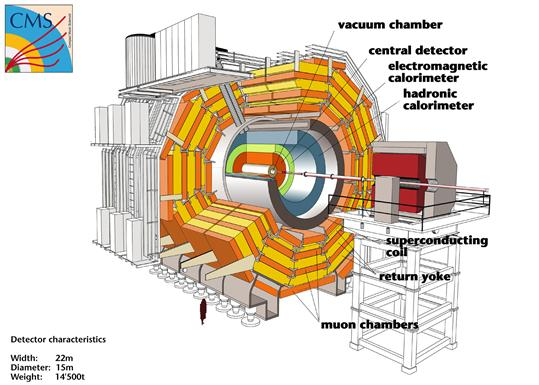
\includegraphics[width=0.7\textwidth]{images/cern-cms-experiment.jpg}
        \caption{The detectors used in the CMS experiment at CERN \cite{cernCmsExperiment}}
    \end{figure}
    
    \section{Particle Identification}
    There are a variety of methods for identifying particles.
    Muons are easily detected as they are the only particles to penetrate into the muon detectors, which are the last stage of the detectors.
    Electrons can be distinguished by causing a shower in the electromagnetic calorimeter, and no corresponding shower in the hadronic calorimeter.
    
    Things get a bit more tricky when it comes to differentiating hadrons, such as pions and kaons.
    One thing we can do is measure the energy loss in silicon trackers.
    It can be shown that this depends on \(\beta \gamma = p/m\).
    We can also measure time of flight using drift chambers or scintillation counters.
    
    Time of flight detectors are particularly useful for particle identification.
    Suppose a particle travels a distance \(L\) at speed \(\beta\), this takes time \(t = L/\beta\).
    We have
    \begin{equation}
        \frac{1}{\beta} = \frac{E}{p} = \frac{\sqrt{p^2 + m^2}}{p} = \sqrt{1 + \frac{m^2}{p^2}} \approx 1 + \frac{m^2}{2p^2}.
    \end{equation}
    We therefore have
    \begin{equation}
        t = L\left( 1 + \frac{m^2}{2p^2} \right).
    \end{equation}
    Suppose an event has the possibility of producing either a kaon or pion, both with equal momentum.
    We can differentiate between the two by considering the time taken to reach a given point a distance \(L\) away from the event.
    In particular the time difference between them arriving is
    \begin{equation}
        \Delta t = \frac{L}{2p^2}(m_{\Pkaon}^2 + m_{\Ppi}^2).
    \end{equation}
    For typically experimental values where \(L\) is on the order of a few metres and \(p\) is on the order of a few \unit{\giga\electronvolt} we find that \(\Delta t\) is on the order of a few hundred pico seconds, which is a measurable time difference, so by measuring momentum and time of flight we can be sure whether we have detected a kaon or pion.
    
    Another effect we can use is \defineindex{Cherenkov} radiation, which is electromagnetic radiation emitted when a particle travels in a medium faster than the speed of light in that medium, essentially the electromagnetic version of a sonic boom.
    The radiation spreads out in a cone, and the angle of the cone depends on \(\beta\).
    Therefore looking at the particle head on we see a ring of Cherenkov radiation, and the radius of this relates to the particle's speed.
    
    Cherenkov radiation can actually be seen by the human eye, and this was used in early accelerators to align beams, by looking down the beam and aligning the beam so that the Cherenkov radiation forms circles, in which case you knew you were looking at it head on.
    Needles to say this is a \emph{bad idea} and if you did it with today's higher energy beams you would almost certainly die.
    
    Astronauts in space (and non-astronauts in space) see flashes of light, which it turns out are due to cherenkov radiation being produced \emph{in their eyes} when particles, mostly from the sun, pass through their eye faster than light travels through their eyes.
    Cherenkov radiation is also seen in water surrounding nuclear detectors, typically the radiation falls in the blue part of the spectrum.
    
    \begin{figure}
        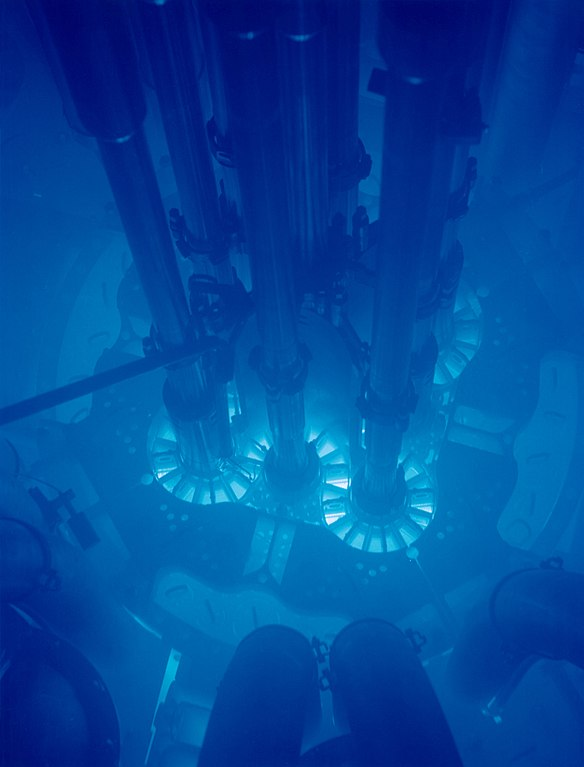
\includegraphics[width=\textwidth]{images/cherenkov-radiation.jpg}
        \caption{Cherenkov radiation in water surrounding a nuclear reactor \cite{cherenkovRadiation}}
    \end{figure}
    
    \section{Neutrinos}
    Neutrinos don't interact in detectors.
    Instead we can infer their presence by looking for \enquote{lost} momentum.
    However, this method can't tell us what the extra, undetected, particle is, just that there is one.
    Most likely the particle is a neutrino, but we can't rule out other non-interacting particles which have yet to be discovered.
    
    \part{Quantum Electrodynamics}
    \chapter{Quantum Electrodynamics}
    \section{Dirac Equation}
    Recall that in \cref{sec:relativistic quantum mechanics} we discussed the Klein-Gordan equation,
    \begin{equation}
        -\diffp[2]{\psi}{t} = -\laplacian\psi + m^2\psi,
    \end{equation}
    which applies to spin zero particles.
    We briefly discussed the existence of negative energy solutions, which we determined correspond to antimatter.
    
    We now briefly cover the \defineindex{Dirac equation}.
    This was found by Dirac, who was dissatisfied with the Klein--Gordan equation.
    He started with the Schr\"odinger-like equation
    \begin{equation}
        i\hbar \diffp{\psi}{t} = \operator{H}\psi
    \end{equation}
    for some Hamiltonian operator \(\operator{H}\).
    Dirac then required that the time and position be treated in the same way, as is common in relativity, this means first order spatial derivatives.
    He concluded that the Hamiltonian must be of the form
    \begin{equation}
        \operator{H} = -i\hbar c\alpha_i\partial_i + \beta mc^2
    \end{equation}
    where we employ the Einstein summation convention summing \(i\) from 1 to 3 in the first term.
    It turns out that \(\alpha_i\), \(\beta\), and \(\psi\) cannot be numbers, but must instead be matrices.
    
    The simplest solution has \(\alpha_i\) and \(\beta\) being \(4 \times 4\) matrices and \(\psi\) being a four component wave-function, known as a spinor.
    The Dirac equation can be written in the form
    \begin{equation}
        \left( i\gamma^0\partial_t + i\vv{\gamma}\cdot\grad - m \right)\psi = (i\gamma^\mu\partial_\mu - m)\psi = 0
    \end{equation}
    where \(\gamma^\mu\) are again \(4\times 4\) constant matrices, which are related to \(\alpha_i\) and \(\beta\) by \(\gamma^0 = \beta\) and \(\gamma^i = \beta\alpha_i\), and we understand that \(\vv{\gamma}\cdot\grad\) is shorthand for
    \begin{equation}
        \vv{\gamma}\cdot\grad = \gamma^i\partial_i = \gamma^1\partial_1 + \gamma^2\partial_2 + \gamma^3\partial_3.
    \end{equation}
    The Dirac equation can be written even more compactly using the Feynman slash notation, where we define \(\slashed{A} \coloneqq \gamma^\mu A_\mu\), so
    \begin{equation}
        (i\slashed{\partial} - m)\psi = 0.
    \end{equation}

    For completeness the gamma matrices, in this four-dimensional representation, are given by
    \begin{alignat}{3}
        \gamma^0 &\coloneqq 
        \begin{bmatrix}
            1 & 0 & 0 & 0\\
            0 & 1 & 0 & 0\\
            0 & 0 & -1 & 0\\
            0 & 0 & 0 & -1
        \end{bmatrix}
        , \qquad &
        \gamma^1 &= 
        \begin{bmatrix}
            0 & 0 & 0 & 1\\
            0 & 0 & 1 & 0\\
            0 & -1 & 0 & 0\\
            -1 & 0 & 0 & 0
        \end{bmatrix}
        ,\\
        \gamma^2 &\coloneqq 
        \begin{bmatrix}
            0 & 0 & 0 & \mathrlap{-i}\hphantom{-1}\\
            0 & 0 & i & 0\\
            0 & i & 0 & 0\\
            \mathrlap{-i}\hphantom{-1} & 0 & 0 & 0
        \end{bmatrix}
        , \qquad &
        \gamma^3 &= 
        \begin{bmatrix}
            0 & 0 & 1 & 0\\
            0 & 0 & 0 & -1\\
            -1 & 0 & 0 & 0\\
            0 & 1 & 0 & 0
        \end{bmatrix}
        .
    \end{alignat}
    These can be compactly written as block matrices:
    \begin{equation}
        \gamma^0 = 
        \begin{bmatrix}
            \ident & 0\\
            0 & -\ident
        \end{bmatrix}
        = \sigma^3 \otimes \ident
        , \qqand
        \gamma^k = 
        \begin{bmatrix}
            0 & \sigma_k\\
            -\sigma_k & 0
        \end{bmatrix}
        = i\sigma^2 \otimes \sigma^k
    \end{equation}
    where \(\otimes\) is the tensor product\footnote{see principles of quantum mechanics notes for more details}, \(\ident\) is the \(2\times 2\) identity matrix and \(\sigma_k\) are the Pauli spin matrices,
    \begin{equation}
        \sigma_1 =
        \begin{bmatrix}
            0 & 1\\
            1 & 0
        \end{bmatrix}
        , \qquad \sigma_2 =
        \begin{bmatrix}
            0 & -i\\
            i & 0
        \end{bmatrix}
        , \qqand \sigma_3 =
        \begin{bmatrix}
            1 & 0\\
            0 & -1
        \end{bmatrix}
        .
    \end{equation}
    
    The Dirac equation has plane wave solutions given by
    \begin{equation}
        \psi(\vv{r}, t) = u(\vv{p}) \exp\left[ -\frac{i}{\hbar} (Et - \vv{r} \cdot \vv{p}) \right]
    \end{equation}
    where \(u\) is some function of the momentum, \(\vv{p}\).
    In four-vector notation and natural units this becomes
    \begin{equation}
        \psi(x^\mu) = u(p^i) \e^{-ix_\mu p^\mu}.
    \end{equation}
    There are still positive and negative energy solutions.
    In fact, there are four solutions, two of which are positive and two of which are negative, once we include spin.
    
    \section{Antimatter}
    The negative energy solutions to the Dirac and Klein--Gordan equation gave rise to the prediction of antimatter.
    There are two common ways to interpret antimatter.
    
    \subsection{Dirac Interpretation}
    Dirac interpreted the negative energy solutions as being hole states.
    That is he imagined that the vacuum is filled with negative energy levels, each of which is occupied by two electrons (with opposite spins).
    This is called the \defineindex{Dirac sea}.
    A hole in the sea then appears as a positively charged state with positive energy.
    From this Dirac predicted the positron in 1928, and it was discovered just a few years later in 1931.
    Note that the energy required to jump from a negative energy state to the positive energy hole state is \(2m_{\Pelectronneutral}c^2\).
    
    \subsection{Feynman--St\"ukelberg Interpretation}
    A more modern view of antimatter is as normal matter moving backwards in time.
    This interpretation is due to the fact that if we have a state,
    \begin{equation}
        \psi(\vv{r}, t) \propto \exp[-i(Et - \vv{r} \cdot \vv{p})],
    \end{equation}
    and we reverse it's direction, so \(\vv{p} \to -\vv{p}\) and time, \(t \to -t\), we get the same state, but moving backwards, so \(\vv{r} \to -\vv{r}\):
    \begin{equation}
        \psi(-\vv{r}, -t) \propto \exp[-i((-E)(-t) - (-\vv{r})\cdot(-\vv{p}))] = \exp[-i(Et - \vv{r}\cdot\vv{p})].
    \end{equation}
    
    \section{Feynman Diagrams}
    \define{Feynman diagrams}\index{Feynman diagram} are a pictorial representation of a process at a particular order in perturbation theory.
    They consist of a directed graph with different types of edges for different types of particles.
    We view time as going from left to right in a Feynman diagram, although other conventions have time flowing upwards.
    A fermion is represented as a straight line with an arrow in the direction of time.
    An antifermion is represented by a straight line with an arrow \emph{backwards} in time.
    A boson is represented by a wavy (photons), loopy (gluons), or dashed (\PW{} and \PZ{} bosons) line.
    This boson line has an arrow only for \PWpm, where the direction the charge is carried is important.
    
    Each Feynman diagram represents a term in a perturbation expansion for a given process.
    This means that there is a set of rules for turning a Feynman diagram into maths, in particular for the matrix element of the term in perturbation theory.
    The set of rules depends on the context of the diagram (QED, QCD, etc.).
    We give the set of rules for QED here:
    \begin{itemize}
        \item A vertex for the interaction of a charged fermion and a photon, the only type of vertex considered in QED, gives a contribution of the charge of the fermion, \(Q\).
        This may also be written in terms of the fine structure constant
        \begin{equation}
            \alpha = \frac{e^2}{4\pi\varepsilon_0\hbar c}
        \end{equation}
        or in natural units, with \(\varepsilon_0 = 1\),
        \begin{equation}
            \alpha = \frac{e^2}{4\pi}.
        \end{equation}
        This is a dimensionless value which is (at low energies\footnote{see \cref{sec:running of alpha}}) approximately \(1/137\).
        So, for fermions with unit magnitude charge we can instead consider a contribution of \(\sqrt{\alpha}\), since these are all just proportionality factors, so the \(1/\sqrt{4\pi}\) can be absorbed in the constant of proportionality.
        \item A photon propagator gives a contribution of \(1/q^2\), where \(q\) is the transferred four-momentum.
    \end{itemize}
    At each vertex charge, momentum, energy, and flavour must be conserved.
    
    A simple first example of a Feynman diagram is an electron scattering off of a muon.
    The Feynman diagram for this is
    \begin{equation}
        \tikzsetnextfilename{electron-muon-scattering}
        \begin{tikzpicture}[baseline=(current bounding box)]
            \begin{feynman}
                \vertex (mu in) {\Pmu};
                \vertex (e in) at (0, 2) {\Pe};
                \vertex (e out) at (4, 2) {\Pe};
                \vertex (mu out) at (4, 0) {\Pmu};
                \vertex (e photon) at (2, 1.5);
                \vertex (mu photon) at (2, 0.5);
                \diagram {
                    (e in) -- [fermion] (e photon) -- [fermion] (e out);
                    (mu in) -- [fermion] (mu photon) -- [fermion] (mu out);
                    (e photon) -- [photon, edge label=\(\Pphoton\), edge label'=\textcolor{highlight}{\(q\)}] (mu photon);
                };
                \node[above] at (e photon) {\textcolor{tetrad blue}{\(e\)}};
                \node[below] at (mu photon) {\textcolor{tetrad purple}{\(e\)}};
            \end{feynman}
        \end{tikzpicture}
    \end{equation}
    The matrix element corresponding to this diagram is
    \begin{equation}
        \matrixelement(\Pe\Pmu\to\Pe\Pmu) \propto \textcolor{tetrad blue}{e}\frac{1}{\textcolor{highlight}{q}^2}\textcolor{tetrad purple}{e} = \frac{e^2}{q^2} \propto \sqrt{\alpha} \frac{1}{q^2} \sqrt{\alpha} = \frac{\alpha}{q^2}.
    \end{equation}

    \subsection{\texorpdfstring{\(\mathsf{s}\), \(\mathsf{p}\), \(\mathsf{u}\)-Channel Diagrams}{s, p, u-Channel Diagrams}}
    For this section we work with examples of \defineindex{Bhabha scattering}, which is the electron-positron scattering process
    \begin{equation}
        \Pe\APe \to \Pe\APe,
    \end{equation}
    as well as electron-electron scattering,
    \begin{equation}
        \Pe\Pe \to \Pe\Pe.
    \end{equation}
    To first order there are three different Feynman diagrams to consider.
    While we refer to the process as scattering this is simply because the initial and final particles are the same.
    We actually have to allow for things like annihilation and then pair production.
    
    \subsubsection{\texorpdfstring{\(\mathsf{s}\)-Channel}{s-Channel}}
    Suppose that the initial electron and positron annihilate, producing a photon, and then that photon produces an electron-positron pair.
    This is shown in the following interaction:
    \begin{equation}
        \tikzsetnextfilename{electron-positron-scattering}
        \begin{tikzpicture}[baseline=(current bounding box)]
            \begin{feynman}
                \vertex (e- in) {\Pe};
                \vertex (e+ in) at (0, 2) {\APe};
                \vertex (annihilate) at (2, 1);
                \vertex (production) at (4, 1);
                \vertex (e- out) at (6, 0) {\Pe};
                \vertex (e+ out) at (6, 2) {\APe};
                \diagram {
                    (e- in) -- [fermion, edge label'=\(p_2\)] (annihilate) -- [photon, edge label=\Pphoton] (production) -- [fermion, edge label'=\(p_4\)] (e- out);
                    (e+ in) -- [anti fermion, edge label=\(p_1\)] (annihilate);
                    (production) -- [anti fermion, edge label=\(p_3\)] (e+ out);
                };
            \end{feynman}
        \end{tikzpicture}
    \end{equation}
    
    For this process we define the quantity \(s\) to be the invariant total four-momentum squared,
    \begin{equation}
        s \coloneqq (p_1 + p_2)^2 = (p_3 + p_4)^2 = q^2,
    \end{equation}
    where \(q\) is the four-momentum of the photon.
    This quantity, \(s\), is one of the three \define{Mandelstam variables}\index{Mandelstam variable}.
    
    This quantity can be defined for any interaction of this type, where two particles combine and then break apart into two new particles.
    We call this an \define{\(\bm{s}\)-channel}\index{s-channel@\(s\)-channel} diagram, where the s stands for space, as the photon is space-like, travelling horizontally, parallel to the time axis.
    
    \subsubsection{\texorpdfstring{\(\mathsf{t}\)-Channel}{t-Channel}}
    Suppose that two electrons scatter, the most obvious way for this to happen is as represented in the following diagram:
    \begin{equation}
        \tikzsetnextfilename{electron-electron-t-scattering}
        \begin{tikzpicture}[baseline=(current bounding box)]
            \begin{feynman}
                \vertex (e1 in) {\Pe};
                \vertex (e2 in) at (0, 2) {\Pe};
                \vertex (e1 photon) at (2, 0.5);
                \vertex (e2 photon) at (2, 1.5);
                \vertex (e1 out) at (4, 0) {\Pe};
                \vertex (e2 out) at (4, 2) {\APe};
                \diagram {
                    (e1 in) -- [fermion, edge label'=\(p_2\)] (e1 photon) -- [fermion, edge label'=\(p_4\)] (e1 out);
                    (e2 in) -- [fermion, edge label=\(p_1\)] (e2 photon) -- [fermion, edge label=\(p_3\)] (e2 out);
                    (e1 photon) -- [photon, edge label=\Pphoton] (e2 photon);
                };
            \end{feynman}
        \end{tikzpicture}
    \end{equation}
    
    For this process we define the quantity \(t\) to be the invariant change in four-momentum squared, so
    \begin{equation}
        t \coloneqq (p_1 - p_3)^2 = (p_2 - p_4)^2 = q^2,
    \end{equation}
    where \(q\) is the four-momentum of the photon.
    This is another one of the Mandelstam variables.
    
    We can define this quantity for any interaction of this type, where one particle emits a particle and the other absorbs it.
    We call this a \define{\(\bm{t}\)-channel}\index{t-channel@\(t\)-channel} diagram, where the \(t\) stands for time, as the photon is time like, travelling vertically, parallel to the space axis.
    
    \subsubsection{\texorpdfstring{\(\mathsf{u}\)-Channel}{u-Channel}}
    The next process is very similar to the previous process.
    Since electrons are all identical we can, in theory, swap the two electrons somewhere along the way and the result should be indistinguishable.
    This is represented by the following diagram:
    \begin{equation}
        \tikzsetnextfilename{electron-electron-u-scattering}
        \begin{tikzpicture}[baseline=(current bounding box)]
            \begin{feynman}
                \vertex (e1 in) {\Pe};
                \vertex (e2 in) at (0, 2) {\Pe};
                \vertex (e1 photon) at (2, 0.5);
                \vertex (e2 photon) at (2, 1.5);
                \vertex (e2 out) at (6, 0) {\Pe};
                \vertex (e1 out) at (6, 2) {\APe};
                \diagram {
                    (e1 in) -- [fermion, edge label'=\(p_2\)] (e1 photon) -- [fermion, edge label=\(p_3\)] (e1 out);
                    (e2 in) -- [fermion, edge label=\(p_1\)] (e2 photon) -- [fermion, edge label'=\(p_4\)] (e2 out);
                    (e1 photon) -- [photon, edge label=\Pphoton] (e2 photon);
                };
            \end{feynman}
        \end{tikzpicture}
    \end{equation}
    
    For this process we define the quantity \(u\) to be the invariant change in four-momentum squared, so
    \begin{equation}
        u \coloneqq (p_1 - p_4)^2 = (p_2 - p_3)^2 = q^2
    \end{equation}
    where \(q\) is the four-momentum of the photon.
    This is the third Mandelstam variable.
    
    We can define this quantity for any interaction of this type, where two identical particles scatter and swap.
    We call this a \define{\(\bm{u}\)-Channel}\index{u-channel@\(u\)-channel} diagram, where the \(u\) stands for \enquote{um, well, the photon is time like but we've already used \(t\), I guess \(u\) is next in the alphabet}.
    
    \section{QED Rules}
    \subsection{QED Vertex}
    The building block of QED is the QED vertex, for example,
    \begin{equation}
        \tikzsetnextfilename{example-QED-vertex}
        \begin{tikzpicture}[baseline=(current bounding box)]
            \begin{feynman}
                \vertex (f1) {\Pfermion};
                \vertex (f2) at (0, 2) {\APfermion};
                \vertex (interaction) at (2, 1);
                \vertex (photon) at (4, 1) {\Pphoton};
                \diagram {
                    (f1) -- [fermion] (interaction) -- [photon] (photon);
                    (f2) -- [anti fermion] (interaction);
                };
            \end{feynman}
        \end{tikzpicture}
    \end{equation}
    This shows a fermion and antifermion annihilating.
    In general a QED vertex involves two charged fermions interacting and then absorption or emission of a photon.
    
    The matrix element corresponding to this vertex is proportional to \(\sqrt{\alpha} \propto e\), where \(\alpha\) is the fine structure constant, and \(e\) is the elementary charge.
    
    At every QED vertex the following must be conserved:
    \begin{itemize}
        \item momentum,
        \item energy,
        \item charge, and
        \item fermion flavour.
    \end{itemize}
    
    Examples of QED vertices are annihilation,
    \begin{equation}
        \tikzsetnextfilename{electron-positron-annihilation-vertex}
        \begin{tikzpicture}[baseline=(current bounding box)]
            \begin{feynman}
                \vertex (e-) {\Pe};
                \vertex (e+) at (0, 2) {\APe};
                \vertex (interaction) at (2, 1);
                \vertex (photon) at (4, 1) {\Pphoton};
                \diagram {
                    (e-) -- [fermion] (interaction) -- [photon] (photon);
                    (e+) -- [anti fermion] (interaction);
                };
            \end{feynman}
        \end{tikzpicture}
    \end{equation}
    pair production,
    \begin{equation}
        \tikzsetnextfilename{electron-positron-production-vertex}\begin{tikzpicture}[baseline=(current bounding box)]
            \begin{feynman}
                \vertex (photon) {\Pphoton};
                \vertex (e-) at (4, -1) {\Pe};
                \vertex (e+) at (4, 1) {\APe};
                \vertex (interaction) at (2, 0);
                \diagram {
                    (photon) -- [photon] (interaction) -- [fermion] (e-);
                    (interaction) -- [anti fermion] (e+);
                };
            \end{feynman}
        \end{tikzpicture}
    \end{equation}
    photon bremsstrahlung,
    \begin{equation}
        \tikzsetnextfilename{photon-bremsstrahlung-vertex}
        \begin{tikzpicture}[baseline=(current bounding box)]
            \begin{feynman}
                \vertex (e- in) {\Pe};
                \vertex (e- out) at (4, -1) {\Pe};
                \vertex (photon) at (4, 1) {\Pphoton};
                \vertex (interaction) at (2, 0);
                \diagram {
                    (e- in) -- [fermion] (interaction) -- [fermion] (e- out);
                    (interaction) -- [photon] (photon);
                };
            \end{feynman}
        \end{tikzpicture}
    \end{equation}
    and photon absorption,
    \begin{equation}
        \tikzsetnextfilename{photon-absorption-vertex}\begin{tikzpicture}[baseline=(current bounding box)]
            \begin{feynman}
                \vertex (e- in) {\Pe};
                \vertex (photon) at (0, 2) {\Pphoton};
                \vertex (interaction) at (2, 1);
                \vertex (e- out) at (4, 1) {\Pe};
                \diagram {
                    (e- in) -- [fermion] (interaction) -- [fermion] (e- out);
                    (photon) -- [photon] (interaction);
                };
            \end{feynman}
        \end{tikzpicture}
    \end{equation}
    
    These are all described by the same basic vertex.
    None of these is a physical process on its own, energy-momentum conservation is violated.
    We need to combine at least two vertices to get a valid physical process.
    
    \section{Perturbation Theory}
    \begin{rmk}
        For more details on basic perturbation theory see the principles of quantum mechanics notes. For details on perturbation theory with path integrals, as used in QFT, and diagrammatic representations of said integrals see the notes from the quantum theory course.
    \end{rmk}
    We said that each Feynman diagram represents a term in perturbation theory to a certain order.
    By this we mean that in a full perturbation theory calculation for the matrix element, \(\matrixelement\), we consider the contribution of all physically allowed diagrams.
    The order of the diagram is simply the power of \(\alpha\) that appears in the associated matrix element, which is now just one term in the sum giving the overall matrix element.
    
    For example, the following diagram is first order in perturbation theory, it has two vertices, each contributing a factor of \(\sqrt{\alpha}\), meaning \(\matrixelement \propto \alpha\), and so \(\abs{\matrixelement}^2 \propto \alpha^2\).
    \begin{equation}\label{eqn:feynman diagram e-e+ annihilation mu- mu+ production}
        \tikzsetnextfilename{first-order-perturbation-example}
        \begin{tikzpicture}[baseline=(current bounding box)]
            \begin{feynman}
                \vertex (annihilate);
                \vertex (e+) at (135:2) {\APe};
                \vertex (e-) at (-135:2) {\Pe};
                \vertex (production) at (2, 0);
                \vertex (mu+) at ($(2, 0) + (45:2)$) {\APmu};
                \vertex (mu-) at ($(2, 0) + (-45:2)$) {\Pmu};
                \diagram {
                    (e+) -- [anti fermion] (annihilate) -- [photon] (production) -- [anti fermion] (mu+);
                    (e-) -- [fermion] (annihilate);
                    (production) -- [fermion] (mu-);
                };
            \end{feynman}
        \end{tikzpicture}
    \end{equation}
    The next two diagrams are both second order in \(\alpha\), having four QED vertices and so \(\abs{\matrixelement}^2 \propto \alpha^4\).
    \begin{gather}
        \tikzsetnextfilename{second-order-perturbation-example-1}
        \begin{tikzpicture}[baseline=(current bounding box)]
            \begin{feynman}
                \vertex (annihilate);
                \vertex (e+) at (135:2) {\APe};
                \vertex (e-) at (-135:2) {\Pe};
                \vertex (e-2) at (-135:1);
                \vertex (production) at (2, 0);
                \vertex (mu+) at ($(2, 0) + (45:2)$) {\APmu};
                \vertex (mu-) at ($(2, 0) + (-45:2)$) {\Pmu};
                \vertex (mu-2) at ($(2, 0) + (-45:1)$);
                \diagram {
                    (e+) -- [anti fermion] (annihilate) -- [photon] (production) -- [anti fermion] (mu+);
                    (e-) -- [fermion] (e-2) -- [fermion] (annihilate);
                    (production) -- [fermion] (mu-2) -- [fermion] (mu-);
                    (e-2) -- [photon] (mu-2);
                };
            \end{feynman}
        \end{tikzpicture}
        \\
        \tikzsetnextfilename{second-order-perturbation-example-2}
        \begin{tikzpicture}[baseline=(current bounding box)]
            \begin{feynman}
                \vertex (annihilate);
                \vertex (e+) at (135:2) {\APe};
                \vertex (e-) at (-135:2) {\Pe};
                \vertex (production) at (2, 0);
                \vertex (mu+) at ($(2, 0) + (45:2)$) {\APmu};
                \vertex (mu+2) at ($(2, 0) + (45:1)$);
                \vertex (mu-) at ($(2, 0) + (-45:2)$) {\Pmu};
                \vertex (mu-2) at ($(2, 0) + (-45:1)$);
                \diagram {
                    (e+) -- [anti fermion] (annihilate) -- [photon] (production) -- [anti fermion] (mu+2) -- [anti fermion] (mu+);
                    (e-) -- [fermion] (annihilate);
                    (production) -- [fermion] (mu-2) -- [fermion] (mu-);
                    (mu-2) -- [photon] (mu+2);
                };
            \end{feynman}
        \end{tikzpicture}
    \end{gather}
    The next two diagrams are third order in \(\alpha\), and so \(\abs{\matrixelement}^2 \propto \alpha^6\).
    \begin{gather}
        \tikzsetnextfilename{third-order-perturbation-example-1}
        \begin{tikzpicture}[baseline=(current bounding box)]
            \begin{feynman}
                \vertex (annihilate);
                \vertex (e+) at (135:2) {\APe};
                \vertex (e-) at (-135:2) {\Pe};
                \vertex (e-2) at (-135:0.75);
                \vertex (production) at (2, 0);
                \vertex (mu+) at ($(2, 0) + (45:2)$) {\APmu};
                \vertex (mu+2) at ($(2, 0) + (45:1)$);
                \vertex (mu+3) at ($(2, 0) + (45:1)$);
                \vertex (mu-) at ($(2, 0) + (-45:2)$) {\Pmu};
                \vertex (mu-2) at ($(2, 0) + (-45:0.75)$);
                \vertex (mu-3) at ($(2, 0) + (-45:1)$);
                \diagram {
                    (e+) -- [anti fermion] (annihilate) -- [photon] (production) -- [anti fermion] (mu+3) -- [anti fermion] (mu+);
                    (e-) -- [fermion] (e-2) -- [fermion] (annihilate);
                    (production) -- [fermion] (mu-2) -- [fermion] (mu-);
                    (e-2) -- [photon] (mu-2);
                    (mu-3) -- [photon] (mu+3);
                };
            \end{feynman}
        \end{tikzpicture}
        \\
        \tikzsetnextfilename{third-order-perturbation-example-2}
        \begin{tikzpicture}[baseline=(current bounding box)]
            \begin{feynman}
                \vertex (annihilate);
                \vertex (e+) at (135:2) {\APe};
                \vertex (e-) at (-135:2) {\Pe};
                \vertex (production) at (2, 0);
                \vertex (production 2) at (0.5, 0);
                \vertex (annihilate 2) at (1.5, 0);
                \vertex (mu+) at ($(2, 0) + (45:2)$) {\APmu};
                \vertex (mu+2) at ($(2, 0) + (45:1)$);
                \vertex (mu-) at ($(2, 0) + (-45:2)$) {\Pmu};
                \vertex (mu-2) at ($(2, 0) + (-45:1)$);
                \diagram {
                    (e+) -- [anti fermion] (annihilate) -- [photon] (production 2);
                    (annihilate 2) -- [photon] (production) [anti fermion] (mu+2) -- [anti fermion] (mu+);
                    (e-) -- [fermion] (annihilate);
                    (production) -- [fermion] (mu-2) -- [fermion] (mu-);
                    (mu-2) -- [photon] (mu+2);
                    (production 2) -- [fermion, half left, edge label=\Pe] (annihilate 2);
                    (production 2) -- [anti fermion, half right, edge label'=\APe] (annihilate 2);
                };
            \end{feynman}
        \end{tikzpicture}
    \end{gather}
    
    In general a graph will have \(\abs{\matrixelement}^2 \propto \alpha^{|V|}\), where \(|V|\) is the number of vertices.
    It can also be shown that an \(2n\)th order diagram, with \(\abs{\matrixelement}^2 \propto \alpha^{2n}\), will have \(n\) loops.
    
    \section{Experimental Tests of QED}
    \subsection{Lamb Shift}
    One of the earliest experimental victories of QED was computing the Lamb shift.
    For hydrogen if we solve the Dirac equation then we would predict that \(2\mathrm{p}_{1/2}\) and \(2\mathrm{s}_{1/2}\) states have the same energy.
    However, if we actually measure the energies of the states we find that the they don't have identical energies.
    QED correctly predicts the small difference in energies if we consider the production of virtual particles, which differs slightly in the two cases as the angular momentums aren't the same.
    
    \subsection{\texorpdfstring{\(\mathsf{g}-2\)}{g - 2}}
    Elementary particles have intrinsic angular momentum through their spin.
    One way of measuring this is to measure the magnetic moment related to the spin.
    We predict that it is given by
    \begin{equation}
        \vv{\mu} = -g\frac{e}{2m}\vv{L},
    \end{equation}
    where \(\vv{L}\) is the electron's angular momentum, \(e\) is the elementary charge, and \(m\) is the electron's mass.
    Classically one would expect that \(g = 1\).
    If we take into account spin, in its most basic form, as in the Stern--Gerlach experiment\footnote{For details on the Stern--Gerlach experiment see the notes from principles of quantum mechanics}, then we find that \(g = 2\).
    Actually measuring the magnetic moment we find that for an electron
    \begin{equation}
        g_{\Pelectronneutral} = 2.00238(6),
    \end{equation}
    which differs from 2 by
    \begin{equation}
        a_{\Pelectronneutral} = \frac{g_{\Pelectronneutral} - 2}{2} \approx \qty{0.1}{\percent}.
    \end{equation}
    To first order in QED we instead predict
    \begin{equation}
        g_{\Pelectronneutral} = 2\left( 1 + \frac{\alpha}{2\pi} \right) \approx 2.00232.
    \end{equation}
    
    A fuller calculation with QED using up to five loops, which corresponds to 12672 diagrams makes predictions that are in remarkable agreement with the measured values:
    \begin{alignat}{3}
        &\text{predicted:}\qquad a_{\Pelectronneutral} = 115965218161(23) \times 10^{-12},\\
        &\text{measured:}\qquad a_{\Pelectronneutral} = 115965218073(28) \times 10^{-12}.
    \end{alignat}
    These agree to within \(2.5\sigma\).
    Feynman famously said
    \begin{displaycquote}{feynmanQED}
        To give you a feeling for the accuracy of these numbers, it comes out something like this: If you were to measure the distance from Los Angeles to New York to this accuracy, it would be exact to the thickness of a human hair.
    \end{displaycquote}
    This was with the numbers as they were in 1985, using the newer numbers above we have about a factor of 10 improvement, meaning that an equivalent statement now would be measuring the distance from New York to Los Angeles to within the width of a red blood cell.
    Alternatively this is approximately equivalent to measuring the circumference of Earth to within the width of a human hair.
    
    
    \section{Running of \texorpdfstring{\(\alpha\)}{alpha}}\index{running of alpha@running of \(\alpha\)}\label{sec:running of alpha}
    The free electron is surrounded by a cloud of virtual particles, including \Pe-\APe{} pairs, due to quantum fluctuations in the vacuum.
    These provide shielding for the real electron.
    This is somewhat analogous to how a positive charge in an otherwise neutral medium induces a charge separation that surrounds it with negative charge, reducing it's effective charge from the outside.
    
    At large distances, which correspond to low energies, an electron is shielded.
    At smaller distances, and higher energies, the shielding is reduced.
    The result is that the effective coupling constant, \(\alpha\), is not actually constant\footnote{the value \(e^2/(4\pi)\) is constant, it's just that at low energies this no longer effectively measures the strength of QED interactions}.
    We say that the value of \(\alpha\) runs.
    
    Consider the interaction in \cref{eqn:feynman diagram e-e+ annihilation mu- mu+ production}.
    This is first order in \(\alpha\), since there are two vertices, both contributing a factor of \(\sqrt{\alpha}\).
    The momentum of the photon, \(q\), is how we measure the energy of the interaction.
    When \(q^2 = 0\) we have \(\alpha = 1/137\).
    When \(q^2 = (\qty{100}{\giga\electronvolt})^2\) we measure \(\alpha = 1/128\).
    
    The value of \(\alpha\) increases with energy, until at some point \(\alpha\) is greater than one.
    At this point we have a problem as the perturbation series that QED calculations are full of no longer converge.
    Fortunately this doesn't happen at any reasonable energy, and it is predicted that gravitational effects will become important at lower energies that the series failing to converge so QED isn't even valid at these energies without modification anyway.
    
    \part{Quantum Chromodynamics}
    \chapter{Introduction to QCD}
    Quantum chromodynamics is the quantum theory of the strong force.
    The strong force is mediated by massless bosons, known as gluons, \(\Pgluon\).
    The strong force equivalent of charge is \defineindex{colour}, which is a property possessed only by quarks and gluons.
    
    \section{Feynman Diagrams}
    \subsection{QCD Vertex}
    The QCD vertex is very similar to that of QED, except that instead of charged fermions we have quarks, and instead of photons we have gluons, which we represent with a loopy line.
    The basic QCD vertex involves a quark and a gluon, for example
    \begin{equation}
        \tikzsetnextfilename{qcd-vertex-example}
        \begin{tikzpicture}[baseline=(current bounding box)]
            \begin{feynman}
                \vertex (annihilate);
                \vertex (q in) {\Pq};
                \vertex (interaction) at (2, 0);
                \vertex (q out) at (4, -1) {\Pq};
                \vertex (g) at (4, 1) {\Pgluon};
                \diagram {
                    (q in) -- [fermion] (interaction) -- [fermion] (q out);
                    (interaction) -- [gluon, edge label=\(q\)] (g);
                };
                \node[below left] at (interaction) {\(\sqrt{\alpha_{\strong}}\)};
            \end{feynman}
        \end{tikzpicture}
    \end{equation}
    
    \subsection{Feynman Rules}
    The Feynman rules for QCD diagrams are almost identical to the QED Feynman rules.
    In QCD the propagator is the gluon, and each propagator of momentum \(q\) leads to a factor of \(1/q^2\) in the matrix element.
    The coupling constant is \(\alpha_{\strong}\), which in analogy with QED we define to be
    \begin{equation}
        \alpha_{\strong} = \frac{g_{\strong}^2}{4\pi} \approx 0.2
    \end{equation}
    where \(g_{\strong}\) is a constant which is somewhat analogous to the charge in QED.
    
    Notice that \(\alpha_{\strong} \approx 0.2\) is significantly larger than the QED equivalent of \(\alpha \approx 0.007\).
    This is because the strong force is stronger than electromagnetism.
    
    \subsection{Examples}
    Since QCD involve quarks, which we only ever see in bound states (see % TODO: add link to colour confinement section
    ), Feynman diagrams tend to be slightly more complicated in QCD.
    For example, the \Pphi{} meson, which is a bound strange and antistrange quark, \Ps\APs, can decay in one of two ways:
    \begin{equation}
        \Pphi \to \PKplus\PKminus, \qqor \Pphi \to \PKzero\APKzero,
    \end{equation}
    which in terms of quark content is
    \begin{equation}
        \Ps\APs \to (\Pu\APs)(\APu\Ps), \qqor \Ps\APs \to (\Pd\APs)(\APd\Ps).
    \end{equation}
    
    These two decays are represented by the following diagrams,
    \begin{equation}
        \tikzsetnextfilename{phi-meson-decay-1}
        \begin{tikzpicture}[baseline=(current bounding box)]
            \begin{feynman}
                \vertex (s in) {\Ps};
                \vertex (as in) at (0, -1) {\APs};
                \vertex (as bend) at (2, -1);
                \vertex (interaction) at (2, 0);
                \vertex (gluon decay) at (3, -0.5);
                \vertex (s out) at (4, 1) {\Ps};
                \vertex (au) at (4, 0) {\APu};
                \vertex (u) at (4, -1) {\Pu};
                \vertex (as out) at (4, -2) {\APs};
                \diagram {
                    (s in) -- [fermion] (interaction) -- [fermion] (s out);
                    (interaction) -- [gluon] (gluon decay) -- [fermion] (u);
                    (gluon decay) -- [anti fermion] (au);
                    (as in) -- [anti fermion] (as bend) -- [anti fermion] (as out);
                };
                \draw[decorate, decoration={brace, amplitude=5pt, mirror, raise=4pt}] (s in.north) -- (as in.south) node[left, midway, xshift=-2ex] {\Pphi};
                \draw[decorate, decoration={brace, amplitude=5pt, raise=4pt}] (s out.north) -- (au.south) node[right, midway, xshift=2ex] {\PKminus};
                \draw[decorate, decoration={brace, amplitude=5pt, raise=4pt}] (u.north) -- (as out.south) node[right, midway, xshift=2ex] {\PKplus};
            \end{feynman}
        \end{tikzpicture}
    \end{equation}
    and
    \begin{equation}
        \tikzsetnextfilename{phi-meson-decay-2}
        \begin{tikzpicture}[baseline=(current bounding box)]
            \begin{feynman}
                \vertex (s in) {\Ps};
                \vertex (as in) at (0, -1) {\APs};
                \vertex (as bend) at (2, -1);
                \vertex (interaction) at (2, 0);
                \vertex (gluon decay) at (3, -0.5);
                \vertex (s out) at (4, 1) {\Ps};
                \vertex (ad) at (4, 0) {\APd};
                \vertex (d) at (4, -1) {\Pd};
                \vertex (as out) at (4, -2) {\APs};
                \diagram {
                    (s in) -- [fermion] (interaction) -- [fermion] (s out);
                    (interaction) -- [gluon] (gluon decay) -- [fermion] (d);
                    (gluon decay) -- [anti fermion] (ad);
                    (as in) -- [anti fermion] (as bend) -- [anti fermion] (as out);
                };
                \draw[decorate, decoration={brace, amplitude=5pt, mirror, raise=4pt}] (s in.north) -- (as in.south) node[left, midway, xshift=-2ex] {\Pphi};
                \draw[decorate, decoration={brace, amplitude=5pt, raise=4pt}] (s out.north) -- (ad.south) node[right, midway, xshift=2ex] {\APKzero};
                \draw[decorate, decoration={brace, amplitude=5pt, raise=4pt}] (d.north) -- (as out.south) node[right, midway, xshift=2ex] {\PKzero};
            \end{feynman}
        \end{tikzpicture}
    \end{equation}
    Notice that in both the antistrange quark isn't actually partaking in the reaction.
    For this reason we may sometimes draw this diagram with just the strange quark, and the two (anti)up quarks, with the implicit second quark in the initial state, since we can't have a single quark on its own.
    
    Another example would be the decay of a \PDeltazero{} hadron, which has quark content \Pu\Pd\Pd, this is essentially an excited neutron with spin \(3/2\).
    This decays to a proton, with quark content \Pu\Pd\Pd, and a negative pion, with quark content \Pd\APu.
    This is represented by the diagram
    \begin{equation}
        \tikzsetnextfilename{delta-zero-decay}
        \begin{tikzpicture}[baseline=(current bounding box)]
            \begin{feynman}
                \vertex (u in) at (0, 4) {\Pu};
                \vertex (d in 1) at (0, 3) {\Pd};
                \vertex (d in 2) at (0, 2) {\Pd};
                \vertex (u out 1) at (4, 4) {\Pu};
                \vertex (d out 1) at (4, 3) {\Pd};
                \vertex (u out 2) at (4, 2) {\Pu};
                \vertex (au out) at (4, 1) {\APu};
                \vertex (d out 2) at (4, 0) {\Pd};
                \vertex (gluon creation) at (2, 1.5);
                \vertex (gluon decay) at (3, 1.5);
                \diagram {
                    (u in) -- [fermion] (u out 1);
                    (d in 1) -- [fermion] (d out 1);
                    (d in 2) -- [fermion] (gluon creation) -- [fermion] (d out 2);
                    (gluon creation) -- [gluon] (gluon decay) -- [fermion] (u out 2);
                    (gluon decay) -- [anti fermion] (au out);
                };
                \draw[decorate, decoration={brace, amplitude=5pt, mirror, raise=4pt}] (u in.north) -- (d in 2.south) node[left, midway, xshift=-2ex] {\PDeltazero};
                \draw[decorate, decoration={brace, amplitude=5pt, raise=4pt}] (u out 1.north) -- (u out 2.south) node[right, midway, xshift=2ex] {\Pp};
                \draw[decorate, decoration={brace, amplitude=5pt, raise=4pt}] (au out.north) -- (d out 2.south) node[right, midway, xshift=2ex] {\Ppizero};
            \end{feynman}
        \end{tikzpicture}
    \end{equation}

    \section{Colour}\label{sec:colour}
    \define{Colour}\index{colour} is the charge of QCD.
    Colour is a conserved quantum number, with three possible values, which we call red (\Predgluon), green (\Pgreengluon), and blue (\Pbluegluon).
    Quarks carry colour, and antiquarks carry anticolour, \APredgluon, \APgreengluon, and \APbluegluon.
    Leptons don't carry colour, and therefore don't interact via the strong force.
    Colour is not like electric charge in that any coloured particle can have posses any colour, it's more like spin in this nature, it's also like spin in the fact that spin has nothing to do with the particle actually rotating, and colour has nothing to do with the particle having a colour in the everyday meaning.
    
    A \defineindex{hadron} is any particle made of quarks.
    They always form such that they are colourless.
    They can do this in one of two ways, firstly they can form \define{mesons}\index{meson}, which are quark-antiquark pairs, in this case the antiquark must have the anticolour of the quark's colour, this gives three options for colours in mesons:
    \begin{equation}
        \Predgluon\APredgluon, \qquad \Pgreengluon\APgreengluon, \qqand \Pbluegluon\APbluegluon.
    \end{equation}
    Secondly, they can form \define{(anti)baryons}\index{baryon}, which are made of three (anti)quarks, all with different colours, so for baryons the colours are \Predgluon\Pgreengluon\Pbluegluon, and for antibaryons the colours are \APredgluon\APgreengluon\APbluegluon.
    
    \begin{figure}
        \tikzsetnextfilename{colour-cancellation}
        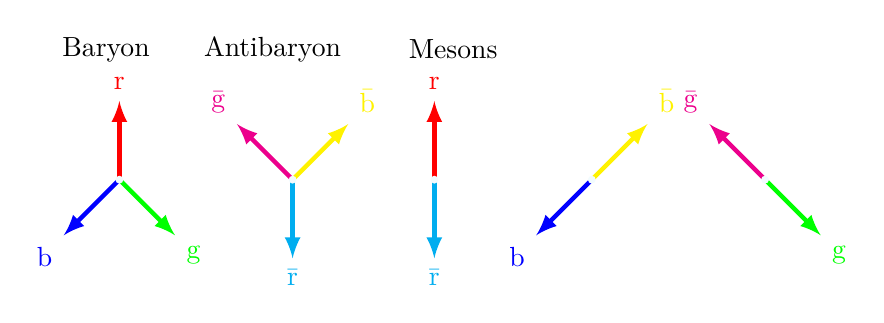
\begin{tikzpicture}
            \draw[ultra thick, ->, red] (0, 0) -- ++ (0, 1) node[above] {\(\mathrm{r}\)};
            \draw[ultra thick, ->, blue] (0, 0) -- ++ (-135:1) node[below left] {\(\mathrm{b}\)};
            \draw[ultra thick, ->, green] (0, 0) -- ++ (-45:1) node[below right] {\(\mathrm{g}\)};
            
            \draw[ultra thick, ->, cyan] (2.2, 0) -- ++ (0, -1)  node[below] {\(\bar{\mathrm{r}}\)};
            \draw[ultra thick, ->, yellow] (2.2, 0) -- ++ (-135:-1)  node[above right] {\(\bar{\mathrm{b}}\)};
            \draw[ultra thick, ->, magenta] (2.2, 0) -- ++ (-45:-1)  node[above left] {\(\bar{\mathrm{g}}\)};
            
            \draw[ultra thick, ->, red] (4, 0) -- ++ (0, 1) node[above] {\(\mathrm{r}\)};
            \draw[ultra thick, ->, cyan] (4, 0) -- ++ (0, -1) node[below] {\(\bar{\mathrm{r}}\)};
            
            \draw[ultra thick, ->, blue] (6, 0) -- ++ (-135:1) node[below left] {\(\mathrm{b}\)};
            \draw[ultra thick, ->, yellow] (6, 0) -- ++ (-135:-1) node[above right] {\(\bar{\mathrm{b}}\)};
            
            \draw[ultra thick, ->, magenta] (8.2, 0) -- ++ (-45:-1) node[above left] {\(\bar{\mathrm{g}}\)};
            \draw[ultra thick, ->, green] (8.2, 0) -- ++ (-45:1) node[below right] {\(\mathrm{g}\)};
            
            \node[right] at ($(-135:1.2) + (0, 2.5)$) {Baryon};
            \node[right] at ($(-135:1.2) + (1.8, 2.5)$) {Antibaryon};
            \node[right] at ($(-135:1.2) + (4.4, 2.5)$) {Mesons};
            
            \foreach \x in {0, 2.2, 4, 6, 8.2} {
                \fill[white!95!cyan] (\x, 0) circle [radius=0.05cm];
            }
        \end{tikzpicture}
        \caption{An intuitive, and completely non-physical, picture explaining why \enquote{colour-anticolour}, and \enquote{all three (anti)colours} are both considered colourless states.}
    \end{figure}

    \section{Gluons}
    The force carriers of the strong force are \define{gluons}\index{gluon}.
    These are massless, electrically neutral, spin 1 bosons, in this regard they behave a lot like photons.
    However, gluons carry colour charge, this means that they also interact through the strong force.
    Gluons carry equal parts colour and anticolour.
    Naively one might expect that as there are 3 colours, and 3 anticolurs, we would have 9 combinations:
    \begin{equation}
        \begin{array}{ccc}
            \Predgluon \APredgluon, & \Predgluon \APgreengluon, & \Predgluon \APbluegluon, \\
            \Pgreengluon \APredgluon, & \Pgreengluon \APgreengluon, & \Pgreengluon \APbluegluon, \\
            \Pbluegluon \APredgluon, & \Pbluegluon \APgreengluon, & \Pbluegluon \APbluegluon.
        \end{array}
    \end{equation}
    However, three of these, \Predgluon\APredgluon, \Pgreengluon\APgreengluon, and \Pbluegluon\APbluegluon, are colourless.
    Instead we see that gluons have colour charge given by linear combinations of these states, for example
    \begin{equation}
        \Predgluon\APgreengluon,\ \Pgreengluon\APredgluon,\ \Predgluon\APbluegluon,\ \Pbluegluon\APredgluon,\ \Pbluegluon\APgreengluon,\ \Pgreengluon\APbluegluon,\ \frac{\sqrt{2}}{2}(\Predgluon\APredgluon - \Pgreengluon\APgreengluon),\ \frac{\sqrt{6}}{6}(\Predgluon\APredgluon + \Pgreengluon\APgreengluon - 2\Pbluegluon\APbluegluon).
    \end{equation}
    We may also expect that we would find a colourless gluon like
    \begin{equation}
        \frac{\sqrt{3}}{3} (\Predgluon\APredgluon + \Pgreengluon\APgreengluon + \Pbluegluon\APbluegluon)
    \end{equation}
    but this isn't the case.
    If this existed it would be a massless, colourless, chargeless, vector boson, and so would behave a lot like photon, in that it wouldn't interact via QCD or QED and would be free, this would give it an infinite range, which we do not observe with the strong force, so we can be certain that this doesn't exist.
    
    \itshape
    From a more abstract point of view QCD is a gauge theory with \(\specialUnitary(3)\) gauge symmetry.
    Gluons are just one representation of this Lie group, so what we mean when we take linear combinations of colours is linear combinations of this representation, which means linear combinations of elements of the general linear group.
    
    There is not just one set of colours that gluons can have, instead we can think of them as a basis for the representation, viewing the general linear group as a vector space, this happens to be an 8-dimensional vector space for this particular representation, which in turn is due to the fact that there are 8 generators of the Lie algebra \(\specialUnitaryLie(3)\), hence there are 8 gluon colour states.
    Importantly the gluon colours we pick must be linearly independent, and must be such that no combination gives one of the forbidden singlet states, which are \Predgluon\APredgluon, \Pgreengluon\APgreengluon, \Pbluegluon\APbluegluon, and \((\Predgluon\APredgluon + \Pbluegluon\APbluegluon + \Pgreengluon\APgreengluon) / \sqrt{2}\).
    
    The requirement that these singlet states be excluded is not one that falls out of the theory, but something that we see in experiments.
    We therefore demand it in our theory.
    If we did see singlet states then we would instead work with the group \(\unitary(3)\), which has one more degree of freedom, and hence an extra state, which would be one of these singlet states, and the others can then be achieved as linear combinations of the 9 basis states.
    \normalfont
    
    In a Feynman diagram we represent gluons as loopy lines if we aren't being specific about colour, if we need to specify colours we can draw a diagram doing so, for example the quark-quark scattering process
    \begin{equation}
        \tikzsetnextfilename{quark-quark-scattering}
        \begin{tikzpicture}[baseline=(current bounding box)]
            \begin{feynman}
                \vertex (q in 1) {\Pq};
                \vertex (q in 2) at (0, 2) {\Pq};
                \vertex (q out 1) at (4, 0) {\Pq};
                \vertex (q out 2) at (4, 2) {\Pq};
                \vertex (interaction 1) at (2, 0.5);
                \vertex (interaction 2) at (2, 1.5);
                \diagram {
                    (q in 1) -- [fermion] (interaction 1) -- [fermion] (q out 1);
                    (q in 2) -- [fermion] (interaction 2) -- [fermion] (q out 2);
                    (interaction 1) -- [gluon] (interaction 2);
                };
            \end{feynman}
        \end{tikzpicture}
    \end{equation}
    may have the colour change as
    \begin{equation}
        \tikzsetnextfilename{quark-quark-scattering-colour}
        \begin{tikzpicture}[baseline=(current bounding box)]
            \begin{feynman}
                \vertex (b in) {\Pbluegluon};
                \vertex (r in) at (0, 2) {\Predgluon};
                \vertex (r out) at (4, 0) {\Predgluon};
                \vertex (b out) at (4, 2) {\Pbluegluon};
                \vertex (r bend 1) at (1.9, 1.5);
                \vertex (r bend 2) at (1.9, 0.5);
                \vertex (b bend 1) at (2.1, 0.5);
                \vertex (b bend 2) at (2.1, 1.5);
                \diagram {
                    (r in) -- [fermion, redgluoncolor] (r bend 1) -- [fermion, redgluoncolor] (r bend 2) -- [fermion, redgluoncolor] (r out);
                    (b in) -- [fermion, bluegluoncolor] (b bend 1) -- [fermion, bluegluoncolor] (b bend 2) -- [fermion, bluegluoncolor] (b out);
                };
            \end{feynman}
        \end{tikzpicture}
    \end{equation}
    Notice that the quark flavour doesn't change, just the colour.
    If we see the gluon as travelling upwards then it is a \Pbluegluon\APredgluon{} gluon, whereas if we see it as travelling downwards then it is a \Predgluon\APbluegluon{} gluon.
    
    \subsection{Self-Interaction}
    Since gluons carry colour they can interact via the strong force.
    For example we can get a three gluon vertex:
    \begin{equation}
        \tikzsetnextfilename{three-gluon-vertex}
        \begin{tikzpicture}[baseline=(current bounding box)]
            \begin{feynman}
                \vertex (gluon 1) {\Pgluon};
                \vertex (interaction) at (2, 0);
                \vertex (gluon 2) at (4, 1) {\Pgluon};
                \vertex (gluon 3) at (4, -1) {\Pgluon};
                \diagram {
                    (gluon 1) -- [gluon] (interaction) -- [gluon] (gluon 2);
                    (interaction) -- [gluon] (gluon 3);
                };
            \end{feynman}
        \end{tikzpicture}
    \end{equation}
    We can also get four gluon vertices.
    
    The existence of these gluon self-interactions makes QCD very different from QED, as we shall soon see.
    
    \section{Colour Confinement}
    In QED we have a potential given by
    \begin{equation}
        V_{\mathrm{QED}} = -\frac{\alpha}{r},
    \end{equation}
    which is the Coulomb potential in units where \(\varepsilon_{0} = 1\).
    At short distances in QCD we have a similar potential,
    \begin{equation}
        V_{\mathrm{QCD}} = -\frac{4}{3}\frac{\alpha_{\strong}}{r}.
    \end{equation}
    
    However, at larger distances self-interactions become more important and the potential actually increases linearly with distance, meaning that at large distances we have a spring like potential
    \begin{equation}
        V_{\mathrm{QCD}} = kr.
    \end{equation}
    This means that we need infinite energy to separate two quarks.
    We call this \defineindex{colour confinement}.
    We can take the potential to be
    \begin{equation}
        V_{\mathrm{QCD}} = -\frac{4}{3}\frac{\alpha_{\strong}}{r} + kr
    \end{equation}
    and calculate the force needed to separate quarks:
    \begin{equation}
        F_{\mathrm{QCD}} = -\diff{V_{\mathrm{QCD}}}{r} = \frac{4}{3}\frac{\alpha_{\strong}}{r} + k.
    \end{equation}
    At large distances we have \(F_{\mathrm{QCD}} \approx k\) and we have measured \(k \approx \qty{1}{\giga\electronvolt\per\femto\metre} \approx \qty{160000}{\newton}\).
    
    In reality what happens when we try to separate two quarks is eventually we put in enough energy that a quark-antiquark pair can be created.
    These will then pair up with the two quarks we were initially trying to separate and the potential energy decreases.
    Quark-antiquark pairs will keep being produced until there is no longer sufficient energy, and we will be left with more quarks, but they will not be separated.
    This process is referred to as hadronisation.
    
    We can use this process to jets of hadrons.
    To do so we need to start with a high energy pair of quarks.
    One way to do this is to start with an electron-positron annihilation:
    \begin{equation}
        \tikzsetnextfilename{electron-positron-annihilate-make-quark-antiquark}
        \begin{tikzpicture}[baseline=(current bounding box)]
            \begin{feynman}
                \vertex (e-) {\Pe};
                \vertex (e+) at (0, 2) {\APe};
                \vertex (annihilate) at (2, 1);
                \vertex (production) at (4, 1);
                \vertex (q) at (6, 2) {\Pq};
                \vertex (aq) at (6, 0) {\APq};
                \diagram {
                    (e-) -- [fermion] (annihilate) -- [photon] (production) -- [fermion] (q);
                    (e+) -- [anti fermion] (annihilate);
                    (production) -- [anti fermion] (aq);
                };
                \node[above right] at (annihilate) {\(Q_{\Pelectronneutral}\)};
                \node[above left] at (production) {\(Q_{\Pq}\)};
            \end{feynman}
        \end{tikzpicture}
    \end{equation}
    This interaction is draw in time and space.
    In just space it looks more like
    \begin{equation}
        \tikzsetnextfilename{electron-positron-create-hadron-jet}
        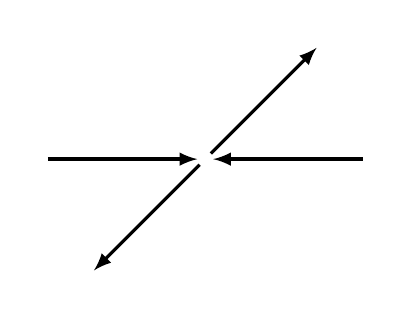
\begin{tikzpicture}[baseline=(current bounding box)]
            \draw[very thick, ->] (-2, 0) node[left] {\Pe} -- (-0.1, 0);
            \draw[very thick, ->] (2, 0) node[right] {\APe} -- (0.1, 0);
            \draw[very thick, ->] (45:0.1) -- (45:2) node[above right] {\Pq};
            \draw[very thick, ->] (-135:0.1) -- (-135:2) node[below left] {\APq};
        \end{tikzpicture}
    \end{equation}
    
    \section{Running of \(\alpha_{\strong}\)}
    For QED we saw that the coupling constant increases with energy due to screening.
    In QCD we also have screening from spontaneous quark-antiquark pair production.
    We also have the effect of gluon pair production.
    This effect provides anti-screening.
    It can be shown that the anti-screening effect of the gluons beats the screening effect of the quarks and \(\alpha_{\strong}\) decreases with distance.
    
    At low energies \(\alpha_{\strong}\) is large and we can't use perturbation theory as the series don't converge.
    At higher energies \(\alpha_{\strong}\) decreases, and eventually it is effectively zero.
    We call this \defineindex{asymptotic freedom}, at sufficiently high energies QCD effects become negligible.
    
    It just so happens that at about \qty{1}{\femto\metre} we have \(\alpha_{\strong} \approx 1\), which means that on the scales of nuclear physics QCD is non-perturbative, and calculations in QCD are very difficult.
    This is why we need high energies, such as those produced in colliders, to study QCD.
    
    \chapter{Tests of QCD}
    \section{Partons}
    In the 1960s many were uncomfortable with the idea of quarks that couldn't be individually observed.
    Feynman proposed a model that served as a stepping stone to the full theory of QCD with quarks and gluons, his idea was that hadrons are made of point like constituent particles, but he made no claim as to what they were.
    He called these particles \define{partons}\index{parton}.
    
    Consider a lepton scattering off of a proton, as in the diagram
    \begin{equation}
        \tikzsetnextfilename{proton-lepton-elastic-scattering}
        \begin{tikzpicture}[baseline=(current bounding box)]
            \begin{feynman}
                \vertex (p in) {\Pp};
                \vertex (p out) at (4, 0) {\Pp};
                \vertex (l in) at (0, 2) {\(\ell^-\)};
                \vertex (l out) at (4, 2) {\(\ell^-\)};
                \vertex (interaction p) at (2, 0.5);
                \vertex (interaction l) at (2, 1.5);
                \diagram {
                    (p in) -- [fermion] (interaction p) -- [fermion] (p out);
                    (l in) -- [fermion] (interaction l) -- [fermion] (l out);
                    (interaction p) -- [photon] (interaction l);
                };
            \end{feynman}
        \end{tikzpicture}
    \end{equation}
    If the particles involved in the scattering are point-like then the cross section is given by the Rutherford scattering formula:
    \begin{equation}
        \diff{\sigma}{\Omega} = \frac{e^4}{4E^2} \frac{\cos^2(\vartheta/2)}{\sin^4(\vartheta/2)}.
    \end{equation}
    
    We can therefore use deviations from this result to probe the inner structure of the proton.
    One example being inelastic scattering, such as
    \begin{equation}
        \tikzsetnextfilename{lepton-proton-inelastic-scattering}
        \begin{tikzpicture}[baseline=(current bounding box)]
            \begin{feynman}
                \vertex (p in) {\Pp};
                \vertex (h out 1) at (4, 0.3);
                \vertex (h out 2) at (4, 0);
                \vertex (h out 3) at (4, -0.3);
                \vertex (l in) at (0, 2) {\(\ell^-\)};
                \vertex (l out) at (4, 2) {\(\ell^-\)};
                \vertex (interaction p) at (2, 0.5);
                \vertex (interaction l) at (2, 1.5);
                \diagram {
                    (p in) -- [fermion] (interaction p) -- [fermion] (h out 1);
                    (interaction p) -- [fermion] (h out 2);
                    (interaction p) -- [fermion] (h out 3);
                    (l in) -- [fermion] (interaction l) -- [fermion] (l out);
                    (interaction p) -- [photon] (interaction l);
                };
                \draw[decorate, decoration={brace, amplitude=5pt, raise=4pt}] (h out 1.north) -- (h out 3.south) node[midway, right, xshift=2ex] {hadrons};
            \end{feynman}
        \end{tikzpicture}
    \end{equation}
    Experimentally we find that the cross section decreases with the momentum transferred, and that the momentum transferred is not constant.
    This is evidence that the proton is not point-like, but has some internal structure.
    Inelastic scattering is particularly useful for this since the result doesn't depend very strongly on the momentum transferred.
    Therefore we can consider very high energy scattering, which we call \defineindex{deep inelastic scattering} and in this regime we see point like scattering, but not off of the proton, off of its point-like constituents, which were thought of as partons in the early experiments.
    
    At relatively low energies the lepton scatters off of the valence quarks, that is the \Pu\Pu\Pd{} quarks that make up the proton.
    At higher energies, which correspond to shorter distances, scattering also occurs from the sea of virtual quarks and gluons that are produced in loops.
    
    We have now performed lepton-proton scattering at wide range of energies and the results are consistent with predictions from QCD.
    In particular we can measure the parton density function, which tells us the probability of finding a parton with given kinematics.
    
    \section{Evidence for Colour}
    \subsection{\PDeltapp{} Baryon}
    The \PDeltapp{} baryon is made of three up quarks, \Pu\Pu\Pu, and has spin \(3/2\), so all three quarks have the same spin.
    The wave function for \PDeltapp{} is symmetric under interchange of identical quarks, since all quarks are the same flavour and spin, which means that the flavour, \(\psi_{\text{flavour}}\), and spin, \(\psi_{\text{spin}}\), factors in the wave function are symmetric.
    However, since \PDeltapp{} is a fermion it must have an antisymmetric wave function.
    This suggests that we are missing a term in the wave function.
    Indeed, we can write the wave function as
    \begin{equation}
        \psi = \psi_{\text{space}}\psi_{\mathrm{flavour}}\psi_{\mathrm{spin}}\psi_{\text{colour}}
    \end{equation}
    where \(\psi_{\text{space}}\), the spatial component of the wave function, is symmetric since the ground state of the \PDeltapp{} baryon has no orbital angular momentum, and so must be spatially symmetric.
    The solution is that the \(\psi_{\text{colour}}\) factor is antisymmetric, which is to say that the quarks all have different colour.
    
    \subsection{\texorpdfstring{\(\Ppizero \to \Pphoton\Pphoton\)}{pi zero to two photons}}
    Consider the interaction \(\Ppizero \to \Pphoton\Pphoton\), recall that the \(\Ppizero\) is made of an up-antiup pair, \Pu\APu.
    This decay is then
    \begin{equation}
        \tikzsetnextfilename{pizero-to-two-photons}
        \begin{tikzpicture}[baseline=(current bounding box)]
            \begin{feynman}
                \vertex (au in) {\APu};
                \vertex (u in) at (0, 2) {\Pu};
                \vertex (a) at (2, 2);
                \vertex (b) at (2, 0);
                \vertex (photon out 1) at (4, 2) {\Pphoton};
                \vertex (photon out 2) at (4, 0) {\Pphoton};
                \diagram {
                    (u in) -- [fermion] (a) -- [fermion] (b);
                    (au in) -- [anti fermion] (b);
                    (a) -- [photon] (photon out 1);
                    (b) -- [photon] (photon out 2);
                };
                \draw[decorate, decoration={brace, amplitude=5pt, raise=4pt}] (au in.south) -- (u in.north) node[midway, left, xshift=-2ex] {\Ppizero};
            \end{feynman}
        \end{tikzpicture}
    \end{equation}
    The width of this interaction is proportional to the number of colours, \(N_c\), squared.
    This comes from considering all possible colours of the two quarks.
    Measurements of \(\Gamma(\Ppizero \to \Pphoton\Pphoton) \propto N_c^2\) gives a value of
    \begin{equation}
        N_c = 2.99 \pm 0.12.
    \end{equation}
    Which is in excellent agreement with the expected value of \(N_c = 3\).
    
    \section{\texorpdfstring{The \(R\)-Ratio}{The R-Ratio}}\label{sec:the R-ratio}\label{sec:R-ratio}
    Consider the two interactions
    \begin{equation}
        \tikzsetnextfilename{electron-positron-to-muons}
        \begin{tikzpicture}[baseline=(current bounding box)]
            \begin{feynman}
                \vertex (e-) {\Pe};
                \vertex (e+) at (0, 2) {\APe};
                \vertex (mu-) at (4.5, 0) {\Pmu};
                \vertex (mu+) at (4.5, 2) {\APmu};
                \vertex (interaction 1) at (1.5, 1);
                \vertex (interaction 2) at (3, 1);
                \diagram {
                    (e-) -- [fermion] (interaction 1) -- [photon] (interaction 2) -- [fermion] (mu-);
                    (e+) -- [anti fermion] (interaction 1);
                    (interaction 2) -- [anti fermion] (mu+);
                };
            \end{feynman}
            \node[above right] at (interaction 1) {\(Q_{\Pe}\)};
            \node[above left] at (interaction 2) {\(Q_{\Pe}\)};
        \end{tikzpicture}
        \text{and}
        \tikzsetnextfilename{electron-positron-to-quarks}
        \begin{tikzpicture}[baseline=(current bounding box)]
            \begin{feynman}
                \vertex (e-) {\Pe};
                \vertex (e+) at (0, 2) {\APe};
                \vertex (mu-) at (4.5, 0) {\Pq};
                \vertex (mu+) at (4.5, 2) {\APq};
                \vertex (interaction 1) at (1.5, 1);
                \vertex (interaction 2) at (3, 1);
                \diagram {
                    (e-) -- [fermion] (interaction 1) -- [photon] (interaction 2) -- [fermion] (mu-);
                    (e+) -- [anti fermion] (interaction 1);
                    (interaction 2) -- [anti fermion] (mu+);
                };
            \end{feynman}
            \node[above right] at (interaction 1) {\(Q_{\Pe}\)};
            \node[above left] at (interaction 2) {\(Q_{\Pq}\)};
        \end{tikzpicture}
    \end{equation}
    For the first interaction \(\matrixelement \propto \alpha/q^2\).
    For the second interaction \(\matrixelement \propto \alpha Q_{\Pq}/q^2\), where \(Q_{\Pq} = 2/3, -1/3\).
    We then define the quantity
    \begin{equation}
        R \coloneqq \frac{\sigma(\Pe\APe \to \text{hadrons})}{\sigma(\Pe\APe \to \Pmu\APmu)} = N_c\sum_i Q_i^2
    \end{equation}
    where \(N_c\) is the number of colours and \(Q_i\) is the energy of the quarks.
    Importantly we sum over only the energetically accessible quarks.
    For an experiment with \(\sqrt{s} \approx \qty{1}{\giga\electronvolt}\) the accessible quarks are \Pu, \Pd, and \Ps.
    Therefore
    \begin{equation}
        R = 3\left( \frac{4}{9} + \frac{1}{9} + \frac{1}{9} \right) = 2.
    \end{equation}
    For \(\sqrt{s} \approx \qty{4}{\giga\electronvolt}\) the charm quark is also accessible and so
    \begin{equation}
        R = 3\left( \frac{4}{9} + \frac{1}{9} + \frac{1}{9} + \frac{4}{9} \right) = \frac{10}{3}.
    \end{equation}
    For \(\sqrt{s} \approx \qty{10}{\giga\electronvolt}\) the bottom quark becomes available and
    \begin{equation}
        R = 3\left( \frac{4}{9} + \frac{1}{9} + \frac{1}{9} + \frac{4}{9} + \frac{1}{9} \right) = \frac{11}{3}.
    \end{equation}
    Finally at \(\sqrt{s} \approx \qty{350}{\giga\electronvolt}\) the top quark becomes available and
    \begin{equation}
        R = 3\left( \frac{4}{9} + \frac{1}{9} + \frac{1}{9} + \frac{4}{9} + \frac{1}{9} + \frac{4}{9} \right) = 5.
    \end{equation}
    We therefore expect that measurements of \(R\) should have discontinuous jumps at energies where new quarks become accessible.
    Further the size of the jumps corresponds to the number of colours and also the charge of the quark that has just become available.
    Indeed, this is exactly what we observe.
    However, the results we observe at lower energies are actually higher than we would predict.
    We will see the reason for this in \cref{sec:running of alpha s}.
    
    \section{Evidence for Gluons}\label{sec:evidence for gluons}
    High energy quarks are likely to emit gluons.
    Like high energy quarks high energy gluons will hadronise and form gets.
    In an interaction producing two quarks we will therefore occasionally see three jets instead of two, if the quarks emit a gluon which creates the third jet.
    The resulting jet pattern is called the \defineindex{Mercedes configuration}, since the three pronged jets resemble the car manufactures' logo.
    
    These jets are observed in particle colliders fairly often and are some of the earliest evidence that gluons exist.
    
    Further, by studying the angles between the highest energy jet and the two other jets it is possible to deduce that the spin of the gluon is 1.
    
    \section{Running of \texorpdfstring{\(\alpha_{\strong}\)}{alpha s}}\label{sec:running of alpha s}
    QCD predicts that \(\alpha_{\strong}\) should decrease with energy.
    We can measure \(\alpha_{\strong}\) with the \(R\)-ratio of \cref{sec:the R-ratio}.
    Recall that this quantity is defined as
    \begin{equation}
        R \coloneqq \frac{\sigma(\Pe\APe \to \text{hadrons})}{\sigma(\Pe\APe \to \Pmu\APmu)}.
    \end{equation}
    In the case where we create hadrons we have to account for these hadrons producing a gluon jet in a three jet event like in \cref{sec:evidence for gluons}.
    \begin{equation}
        \tikzsetnextfilename{electron-positron-3-jet-event}
        \begin{tikzpicture}[baseline=(current bounding box)]
            \begin{feynman}
                \vertex (e-) {\Pe};
                \vertex (e+) at (0, 2) {\APe};
                \vertex (q) at (4.5, 0) {\Pq};
                \vertex (aq midway) at (3.75, 1.5);
                \vertex (aq) at (4.5, 2) {\APq};
                \vertex (g) at (4.5, 1) {\Pgluon};
                \vertex (interaction 1) at (1.5, 1);
                \vertex (interaction 2) at (3, 1);
                \diagram {
                    (e-) -- [fermion] (interaction 1) -- [photon] (interaction 2) -- [fermion] (q);
                    (e+) -- [anti fermion] (interaction 1);
                    (interaction 2) -- [anti fermion] (aq midway) -- [anti fermion] (aq);
                    (aq midway) -- [gluon] (g);
                };
            \end{feynman}
            \node[above right] at (interaction 1) {\(Q_{\Pe}\)};
            \node[above left] at (interaction 2) {\(Q_{\Pq}\)};
            \node[above left] at (aq midway) {\(\sqrt{\alpha_{\strong}}\)};
        \end{tikzpicture}
    \end{equation}
    If we account for these then we find that
    \begin{equation}
        R = N_c\sum_i Q_i^2\left( 1 + \frac{\alpha_{\strong}}{\pi} \right).
    \end{equation}
    The extra factor in the sum is
    \begin{equation}
        1 + \frac{\alpha_{\strong}}{\pi} \approx \frac{3.85}{3.66} \approx 1.05
    \end{equation}
    at \(\qty{25}{\giga\electronvolt}\).
    
    We see this in the data at lower energies.
    We find that \(R\) is larger than the theoretical prediction from first order diagrams.
    At higher energies \(\alpha_{\strong}\) decreases and the data comes in line with the theory as the second order diagrams become less important.
    
    Another useful ratio is the ratio of cross sections for 3-jet events to 2-jet events
    \begin{equation}
        R_3 \coloneqq \frac{\sigma(\Pe\APe \to \text{3-jets})}{\sigma(\Pe\APe \to \text{2-jets})} \propto \alpha_{\strong}.
    \end{equation}
    This also decreases with energy, as expected.
    
    \chapter{Isospin and Hadron Spectroscopy}
    In the 1950s and 1960s many new particle states were discovered.
    We now understand these to be simply combinations of fundamental particles, such as quarks.
    But it is still advantageous to study these particle states with the concepts that were discovered at the same time.
    Two of these concepts being parity and isospin.
    
    \section{Parity}
    The parity operator, \(P\), has the action of replacing \(\vv{r}\) with \(-\vv{r}\) in the wave function:
    \begin{equation}
        P\ket{\psi(\vv{r}, t)} = \ket{\psi(-\vv{r}, t)}.
    \end{equation}
    The \defineindex{parity} of a state is the eigenvalue associated with this operator.
    The parity of a proton is 1 and the parity of a neutron is \(-1\).
    An antifermion will have the opposite parity to its fermion counterpart.
    Bosons and antibosons will have the same parity.
    
    Ground states have an intrinsic parity, which is the parity mentioned above for the proton and neutron.
    For states with angular momentum, \(\ell\), there is also an additional term \((-1)^{\ell}\).
    
    We classify particles into one of four types based on their angular momentum, \(J\), and parity, \(P\), which we denote \(\pm\) for \(\pm 1\).
    \begin{description}
        \item[Scalar] \(J^P = 0^+\),
        \item[Pseudoscalar] \(J^P = 0^-\),
        \item[Vector] \(J^P = 1^-\), and
        \item[Pseudovector] \(J^P = 1^+\).
    \end{description}
    
    A meson will have overall parity \(P_{\Pq}P_{\APq}(-1)^{\ell}\), where \(P_{\Pq}\) and \(P_{\APq}\) are the parities of the quark and antiquark and \(\ell\) is the angular momentum.
    
    Parity is conserved in the strong and electromagnetic interactions, but not in the weak interaction.
    
    \section{Isospin}
    The concept of isospin was first introduced by Heisenberg to explain why protons and neutrons are interchangeable in strong and weak interactions.
    It was later expanded to other concepts.
    Since it was proposed before we knew of quarks it has a somewhat clunky relation to more modern concepts.
    We define the \defineindex{isospin}, \(\ket{I,I_3}\), of a particle to be such that
    \begin{equation}
        I_3 \coloneqq \frac{1}{2}(N_{\Pu} - N_{\Pd})
    \end{equation}
    and \(I\) is the maximum value of \(I_3\) in the same multiplet.
    Recall that \(N_{\Pq}\) is the number of quarks of type \(\Pq\) and that antiquarks of type \(\APq\) count as negative.
    Multiplets themselves are an idea that is beyond the scope of the course but we can think of them as ways of grouping particles.
    For example the pions, \Ppiplus, \Ppizero, and \Ppiminus, form a triplet:
    \begin{align}
        \Ppiplus (\Pu\APd): \ket{I, I_3} = \ket{11}, \qquad &\Ppizero (\Pu\APu): \ket{I, I_3} = \ket{10},\\
        \text{and}\qquad &\Ppiminus (\APu\Pd): \ket{I, I_3} = \ket{1,{-1}}.
    \end{align}
    We also have a duplet of the proton and neutron:
    \begin{equation}
        \Pp (\Pu\Pu\Pd): \ket{I, I_3} = \ket*{\frac{1}{2}\frac{1}{2}}, \qqand \Pn (\Pu\Pd\Pd): \ket{I, I_3} = \ket*{\frac{1}{2},-\frac{1}{2}}.
    \end{equation}
    We consider a quadruplet of delta baryons:
    \begin{align}
        \PDeltapp(\Pu\Pu\Pu) : \ket{I,I_3} = \ket*{\frac{3}{2}\frac{3}{2}}, \qquad & \PDeltap(\Pu\Pu\Pd) : \ket{I,I_3} = \ket*{\frac{1}{2}\frac{3}{2}},\\
        \PDeltazero(\Pu\Pd\Pd) : \ket{I,I_3} = \ket*{\frac{3}{2},-\frac{1}{2}}, \qquad & \PDeltam(\Pd\Pd\Pd) : \ket{I,I_3} = \ket*{\frac{3}{2},-\frac{3}{2}}.
    \end{align}
    
    We can define the \defineindex{hypercharge} as \(Y \coloneqq \baryonnumber + S\) where \(\baryonnumber\) is the baryon number and \(S = N_{\Ps} - N_{\APs}\) is the strangeness quantum number.
    It then turns out that \(I_3 = Q - Y/2\) where \(Q\) is the charge.
    
    The concept of isospin is useful because it allows us to predict properties.
    For example the particle \(\upSigma^+(1189)\) particle, which we now know has quark content \Pu\Pu\Ps, was first observed in the strong interaction
    \begin{equation}
        \PKminus + \Pp \to \Ppiminus + \upSigma^+(1189).
    \end{equation}
    This particle decays by one of two modes
    \begin{equation}
        \upSigma^+(1189) \to \Ppiplus + \Pn, \Ppizero + \Pp.
    \end{equation}
    Since the strong interaction conserves strangeness and baryon number, and on the left in the interaction we have \(\baryonnumber = 1\) and \(S = -1\), it follows that \(Y = 0\) and \(I_3 = Q = 1\).
    Since \(I_3 \ne 0\) we can predict the existence of other particles in the same isospin multiplet with \(I_3 = Q = 0, -1\).
    
    One of the early victories of particle physics was finding a way to group particles such that we can predict the existence of missing particles.
    For example one way of arranging hadrons in a way consistent with the underlying symmetries is given in \cref{fig:grouping hadrons 1,fig:grouping hadrons 2}.
    The grouping in \cref{fig:grouping hadrons 2} allowed Murray Gell-Mann to predict the existence of the \(\upOmega^-\) baryon before it was found experimentally.
    
    \begin{figure}
        \begin{subfigure}{0.5\textwidth}
            \centering
            \tikzsetnextfilename{pseudoscalar-nonet}
            \begin{tikzpicture}
                \draw[thick, ->] (-2.6, 0) node[left] {\hphantom{\(I_3\)}} -- (2.6, 0) node[right] {\(I_3\)};
                \draw[thick, ->] (0, -2.2) -- (0, 2.2) node[above] {\(S\)};
                
                \node[fill=white] (centre) at (0, 0) {\(\upeta\), \(\upeta'\), \Ppizero};
                \node[fill=white] (a) at (0:2) {\Ppiplus};
                \node (b) at (60:2) {\PKplus};
                \node (c) at (120:2) {\PKzero};
                \node[fill=white] (d) at (180:2) {\Ppiminus};
                \node (e) at (240:2) {\PKminus};
                \node (f) at (300:2) {\APKzero};
                
                \foreach \nd in {a, b, c, d, e, f} \draw[highlight, very thick] (centre) -- (\nd);
                \draw[highlight, very thick] (a) -- (b) -- (c) -- (d) -- (e) -- (f) -- (a);
            \end{tikzpicture}
            \caption{The pseudoscalar (\(J^P = 0^-\)) nonet.}
        \end{subfigure}
        \begin{subfigure}{0.5\textwidth}
            \centering
            \tikzsetnextfilename{vector-nonet}
            \begin{tikzpicture}
                \draw[thick, ->] (-2.6, 0) node[left] {\hphantom{\(I_3\)}} -- (2.6, 0) node[right] {\(I_3\)};
                \draw[thick, ->] (0, -2.2) -- (0, 2.2) node[above] {\(S\)};
                
                \node[fill=white] (centre) at (0, 0) {\(\upomega^0\), \(\Pphi\), \(\uprho^0\)};
                \node[fill=white] (a) at (0:2) {\(\uprho^+\)};
                \node (b) at (60:2) {\(\mathrm{K}^{*+}\)};
                \node (c) at (120:2) {\(\mathrm{K^{*0}}\)};
                \node[fill=white] (d) at (180:2) {\(\uprho^-\)};
                \node (e) at (240:2) {\(\mathrm{K}^{*-}\)};
                \node (f) at (300:2) {\(\overline{\mathrm{K}^{*0}}\)};
                
                \foreach \nd in {a, b, c, d, e, f} \draw[highlight, very thick] (centre) -- (\nd);
                \draw[highlight, very thick] (a) -- (b) -- (c) -- (d) -- (e) -- (f) -- (a);
            \end{tikzpicture}
            \caption{The vector (\(J^P = 1^-\)) nonet.}
        \end{subfigure}
        \begin{subfigure}{0.5\textwidth}
            \centering
            \tikzsetnextfilename{octet}
            \begin{tikzpicture}
                \draw[thick, ->] (-2.6, 1.73) node[left] {\hphantom{\(I_3\)}} -- (2.6, 1.73) node[right] {\(I_3\)};
                \draw[thick, ->] (0, -2.2) -- (0, 2.2) node[above] {\(S\)};
                
                \node[fill=white] (centre) at (0, 0) {\(\upSigma^0\), \(\upLambda^0\)};
                \node (a) at (0:2) {\(\upSigma^+\)};
                \node[fill=white] (b) at (60:2) {\Pp};
                \node[fill=white] (c) at (120:2) {\Pn};
                \node (d) at (180:2) {\(\upSigma^-\)};
                \node (e) at (240:2) {\(\upXi^-\)};
                \node (f) at (300:2) {\(\upXi^0\)};
                
                \foreach \nd in {a, b, c, d, e, f} \draw[highlight, very thick] (centre) -- (\nd);
                \draw[highlight, very thick] (a) -- (b) -- (c) -- (d) -- (e) -- (f) -- (a);
            \end{tikzpicture}
            \caption{The \(J^P = \tfrac{1}{2}^+\) octet.}
        \end{subfigure}
        \caption{Grouping hadrons.}
        \label{fig:grouping hadrons 1}
    \end{figure}
    \begin{figure}
        \tikzsetnextfilename{decuplet}
        \begin{tikzpicture}
            \draw[thick, ->] (-3.5, 1.73) node[left] {\hphantom{\(I_3\)}} -- (3.5, 1.73) node[right] {\(I_3\)};
            \draw[thick, ->] (0, -3.8) -- (0, 2.2) node[above] {\(S\)};
            
            \node[fill=white, inner sep=1pt] (centre) at (0, 0) {\(\hphantom{^{*0}}\upSigma^{*0}\)};
            \node (a) at (0:2) {\(\upSigma^{*+}\)};
            \node[fill=white] (b) at (60:2) {\PDeltap};
            \node[fill=white] (c) at (120:2) {\PDeltazero};
            \node (d) at (180:2) {\(\upSigma^{*-}\)};
            \node (e) at (240:2) {\(\upXi^{*-}\)};
            \node (f) at (300:2) {\(\upXi^{*0}\)};
            \node[fill=white] (g) at (30:{2*sqrt(3)}) {\PDeltapp};
            \node[fill=white] (h) at (150:{2*sqrt(3)}) {\PDeltam};
            \node[fill=white] (i) at (270:{2*sqrt(3)}) {\(\hphantom{^-}\upOmega^-\)};
            
            \foreach \nd in {a, b, c, e, f} \draw[highlight, very thick] (centre) -- (\nd);
            \draw[highlight, very thick] (d) -- ++ (1.8, 0);
            \draw[highlight, very thick] (a) -- (b) -- (c) -- (d) -- (e) -- (f) -- (a);
            \draw[highlight, very thick] (a) -- (g) -- (b);
            \draw[highlight, very thick] (c) -- (h) -- (d);
            \draw[highlight, very thick] (e) -- (i) -- (f);
        \end{tikzpicture}
        \caption{More hadron grouping, the \(J^P = \tfrac{3}{2}^+\) decuplet.}
        \label{fig:grouping hadrons 2}
    \end{figure}
    
    \section{Charmonium}
    \subsection{The November Revolution}
    In the early 1970s the idea of quarks was starting to be accepted, and the notion of colour and QCD was starting to be developed, although it was far from being accepted as the theory of the strong force.
    In 1974 the Mark I detector at SLAC the Stanford's positron electron accelerating ring collider (SPEAR)\glossary[acronym]{SPEAR}{Stanford's positron electron accelerating ring collider}, while studying the \(R\) ratio, of \cref{sec:R-ratio}, in the previously unexplored region around \(\sqrt{s} = \qty{3}{\giga\electronvolt}\) a signal was discovered.
    First discovered in a broad scan they decided to go back and look more carefully.
    They found that the signal appeared at a beam energy of \qty{1.56}{\giga\electronvolt}, and vanished when the beam energy was reduced to \qty{1.55}{\giga\electronvolt}, reappearing at \qty{1.555}{\giga\electronvolt}.
    This very narrow resonance corresponds to a new meson.
    
    \subsection{The \texorpdfstring{\PJpsi}{J/psi}}
    The particle that they had observed is now known as the \PJpsi, the reason for the odd name being that the same particle was discovered at Brookhaven around the same time and both experiments gave it a different name, Brookhaven going for J, and SLAC for \(\uppsi\).
    
    We now know that the \PJpsi{} is a bound charmonium state, that is a charm-anticharm, \Pc\APc.
    It has an angular momentum of 1, since it is produced from the decay of a photon.
    Our current best measurement of its mass is \qty{3.0969}{\giga\electronvolt}.
    The observed width, of approximately \qty{3}{\mega\electronvolt}, is mostly due to limited experimental resolution.
    The resonance is actually extremely narrow and is predicted to have width \(\Gamma_{\PJpsi} \approx \qty{93}{\kilo\electronvolt}\).
    
    The \PJpsi{} can decay either to hadrons or to leptons, with branching fractions
    \begin{gather}
        \branchingfraction(\PJpsi \to \text{hadrons}) = 0.88,\\ \branchingfraction(\PJpsi \to \Pe\APe) \approx \branchingfraction(\PJpsi \to \Pmu\APmu) \approx 0.06.
    \end{gather}
    Note that \(2m_{\Ptauneutral} = \qty{3.55}{\giga\electronvolt} > m_{\PJpsi}\), so \(\PJpsi \to \Ptau\APtau\) cannot occur.
    
    While \PJpsi{} has an angular momentum of 1, due to its method of production, there are other bound \Pc\APc{} states with different quantum numbers.
    We find these at slightly different masses in a range from approximately \qtyrange{3}{4.5}{\giga\electronvolt}.
    
    The \PJpsi{} is very narrow, the reason for this is it would \enquote{like} to decay to \(\mathrm{D}^+\mathrm{D}^-\), which are mesons consisting of \Pc\APd{} and \Pd\APc{} respectively,
    \begin{equation}
        \tikzsetnextfilename{Jpsi-forbidden-decay}
        \begin{tikzpicture}[baseline=(current bounding box)]
            \begin{feynman}
                \vertex (ac in) {\APc};
                \vertex (c in) at (0, 2) {\Pc};
                \vertex (ac out) at (4, 0) {\APc};
                \vertex (c out) at (4, 2) {\Pc};
                \vertex (emit g) at (2, 2);
                \vertex (g decay) at (3, 1);
                \vertex (ad out) at (4, 1.5) {\APd};
                \vertex (d out) at (4, 0.5) {\Pd};
                \diagram {
                    (ac in) -- [anti fermion] (ac out);
                    (c in) -- [fermion] (emit g) -- [fermion] (c out);
                    (emit g) -- [gluon] (g decay) -- [fermion] (d out);
                    (g decay) -- [anti fermion] (ad out);
                };
            \end{feynman}
            \draw[decorate, decoration={brace, amplitude=5pt, raise=4pt}] (ac in.south) -- (c in.north) node[midway, left, xshift=-2ex] {\PJpsi};
            \draw[decorate, decoration={brace, amplitude=5pt, raise=4pt}] (c out.north) -- (ad out.south) node[midway, right, xshift=2ex] {\(\mathrm{D}^+\)};
            \draw[decorate, decoration={brace, amplitude=5pt, raise=4pt}] (d out.north) -- (ac out.south) node[midway, right, xshift=2ex] {\(\mathrm{D}^-\)};
        \end{tikzpicture}
    \end{equation}
    however, this is kinematically forbidden as
    \begin{equation}
        2m_{\mathrm{D}} = \qty{3.739}{\giga\electronvolt} > m_{\PJpsi}.
    \end{equation}
    Above a certain energy, known as the open charm threshold, this decay becomes accessible, for example, the \(\uppsi(3770)\) state can decay this way (3370 here being the mass in \unit{\mega\electronvolt}).
    This state has a much wider resonance.
    
    Instead of this decay the \PJpsi{} must decay to lighter mesons, for example an allowed decay is
    \begin{equation}
        \tikzsetnextfilename{Jpsi-allowed-decay-to-pions}
        \begin{tikzpicture}[baseline=(current bounding box)]
            \begin{feynman}
                \vertex (ac in) {\APc};
                \vertex (c in) at (0, 2) {\Pc};
                \vertex (a) at (2, 2);
                \vertex (b) at (2, 0);
                \vertex (g1 emit) at (2, 1.5);
                \vertex (g2 emit) at (2, 1);
                \vertex (g3 emit) at (2, 0.5);
                \vertex (g1 decay) at (4, 1.5);
                \vertex (g2 decay) at (2.75, 1);
                \vertex (g3 decay) at (4, 0.5);
                \vertex (u out) at (5, 2.5) {\Pu};
                \vertex (ad1 out) at (5, 2) {\APd};
                \vertex (d1 out) at (5, 1.25) {\Pd};
                \vertex (ad2 out) at (5, 0.75) {\APd};
                \vertex (d2 out) at (5, 0) {\Pd};
                \vertex (au out) at (5, -0.5) {\Pu};
                \diagram {
                    (c in) -- [fermion] (a) -- (b);
                    (ac in) -- [anti fermion] (b);
                    (g1 emit) -- [gluon] (g1 decay);
                    (g2 emit) -- [gluon] (g2 decay);
                    (g3 emit) -- [gluon] (g3 decay);
                    (g1 decay) -- [anti fermion] (ad1 out);
                    (g1 decay) -- [fermion] (d1 out);
                    (g2 decay) -- [fermion] (u out);
                    (g2 decay) -- [anti fermion] (au out);
                    (g3 decay) -- [anti fermion] (ad2 out);
                    (g3 decay) -- [fermion] (d2 out);
                };
            \end{feynman}
            \draw[decorate, decoration={brace, amplitude=5pt, raise=4pt}] (ac in.south) -- (c in.north) node[midway, left, xshift=-2ex] {\PJpsi};
            \draw[decorate, decoration={brace, amplitude=5pt, raise=4pt}] (u out.north) -- (ad1 out.south) node[midway, right, xshift=2ex] {\(\Ppiplus\)};
            \draw[decorate, decoration={brace, amplitude=5pt, raise=4pt}] (d1 out.north) -- (ad2 out.south) node[midway, right, xshift=2ex] {\(\Ppizero\)};
            \draw[decorate, decoration={brace, amplitude=5pt, raise=4pt}] (d2 out.north) -- (au out.south) node[midway, right, xshift=2ex] {\(\Ppiminus\)};
        \end{tikzpicture}
    \end{equation}
    This is suppressed by the \defineindex{Zweig rule}, which states that decays in which the Feynman diagram separates into two disconnected components upon removing the gluon lines such that the initial particles are disconnected from the final particles are suppressed.
    We need three gluons to conserve colour, and so \(\matrixelement\propto \alpha_{\strong}^3\).
    Further the gluons have to be massive, as they need to carry away the approximately \qty{3}{\giga\electronvolt}, of mass from the quarks.
    This further suppresses this decay as \(\alpha_{\strong}\) runs, and therefore decreases.
    The combined effect of this suppression is a very narrow resonance.
    
    \section{Other QCD States}
    Since the 1970s when charmonium was first observed we have also found bottomomium states, which are bound \Pb\APb{} states.
    Measurements of these states agree well with predictions of QCD.
    
    More interestingly we have also observed states with more than 3 quarks.
    This includes tetraquarks, which are made of two quarks and two antiquarks, essentially forming bound meson-meson pairs, and pentaquarks, which are made of four quarks and an antiquark, essentially forming a bound meson-baryon pair.
    The existence of hexaquarks, made from either 6 quarks in a bound dibaryon state, or 3 quarks and 3 antiquarks, in a bound 3 meson state, has also been hypothesised.
    
    Another prediction of QCD is the existence of glueballs, which are bound states consisting solely of gluons, with no quarks.
    It's predicted that such states could be detected at current collider energies but identifying these states would be incredibly difficult.
    There are some candidate particles that it is thought might be glueballs but this has not yet been confirmed.
    
    We are still actively finding new hadronic resonances regularly.
    A recent example being \(\mathrm{T}_{\Pc\Pc}^+\), with quark content \Pc\Pc\APu\APd, which decays to \(\mathrm{D}^0\mathrm{D}^0\Ppiplus\), where \(\mathrm{D}^{0}\) has quark content \Pc\APu.
    It is not yet known whether \(\mathrm{T}_{\Pc\Pc}^+\) is a tetra quark or a bound \(\mathrm{D^0}\mathrm{D^{+*}}\) pair of mesons, \(\mathrm{D}^{+*}\) has quark content \Pc\APd.
    
    \part{The Weak Force}
    \chapter{The Weak Interaction}
    \section{The Basics}
    The weak interaction is responsible for
    \begin{itemize}
        \item muon and tau decay,
        \item light hadron decay,
        \item nuclear fission and fusion,
        \item neutrino interactions.
    \end{itemize}
    The weak force is, as the name suggests, weak.
    Cross sections for weak processes are small, on the order of \(10^{-13}\,\unit{\milli\barn}\), and lifetimes are relatively long, on the order of \(10^{-13}\,\unit{\second}\)--\(10^{3}\,\unit{\second}\).
    
    There are two types of weak interactions.
    Neutral current processes are mediated by \PZ{} bosons, which have mass \(m_{\PZ} = \qty{91.2}{\giga\electronvolt}\).
    Charged current processes are mediated by \PW{} bosons, which have charge \(\pm 1\), and mass \(m_{\PW} = \qty{80.4}{\giga\electronvolt}\).
    
    The \PZ{} boson interacts with all quarks and all leptons, including neutrinos.
    It doesn't change fermion flavour.
    The \PW{} boson interacts with all quarks and leptons, including neutrinos, and it can change fermion flavour.
    In general in a process involving a photon we can replace the photon with a \PZ{} boson, although not vice-versa as photons don't interact with neutrinos.
    
    \PZ{} and \PW{} can also interact with each other, for example,
    \begin{equation}
        \tikzsetnextfilename{Z-decay-to-W}
        \begin{tikzpicture}[baseline=(current bounding box)]
            \begin{feynman}
                \vertex (Z) {\PZ};
                \vertex (decay) at (2, 0);
                \vertex (W+) at (4, 1) {\PWp};
                \vertex (W-) at (4, -1) {\PWm};
                \diagram {
                    (Z) -- [boson] (decay) -- [boson] (W+);
                    (decay) -- [boson] (W-);
                };
            \end{feynman}
        \end{tikzpicture}
    \end{equation}
    another way of creating two \PW{} bosons is through a photon decaying:
    \begin{equation}
        \tikzsetnextfilename{Z-decay-to-W}
        \begin{tikzpicture}[baseline=(current bounding box)]
            \begin{feynman}
                \vertex (photon) {\Pphoton};
                \vertex (decay) at (2, 0);
                \vertex (W+) at (4, 1) {\PWp};
                \vertex (W-) at (4, -1) {\PWm};
                \diagram {
                    (photon) -- [boson] (decay) -- [boson] (W+);
                    (decay) -- [boson] (W-);
                };
            \end{feynman}
        \end{tikzpicture}
    \end{equation}
    
    \section{Feynman Rules}
    The Feynman rules for the weak interaction are more complicated than for QED or QCD since there are multiple massive bosons.
    The coupling strength depends on the boson, with each weak vertex contributing \(g_{\PW} \propto \sqrt{\alpha_{\PW}}\) for charged weak currents, or \(g_{\PZ} \propto \sqrt{\alpha_{\PZ}}\) for neutral weak currents.
    Each propagator then contributes
    \begin{equation}
        \frac{1}{q^2 - m_{\PW}^2}, \qqor \frac{1}{q^2 - m_{\PZ}^2}
    \end{equation}
    for charged and neutral weak currents respectively.
    Compare this to the propagator term in QED and QCD of \(1/q^2\), since the exchange particles are massless in these theories.
    
    For charged interactions involving quarks there is one more complexity, the coupling strength depends on the quarks.
    We will see this more later, for now in the interaction
    \begin{equation}
        \tikzsetnextfilename{W-quark-flavour-change-vertex}
        \begin{tikzpicture}[baseline=(current bounding box)]
            \begin{feynman}
                \vertex (q) {\Pq};
                \vertex (decay) at (2, 0);
                \vertex (q') at (4, 1) {\Pq'};
                \vertex (W) at (4, -1) {\PW};
                \diagram {
                    (q) -- [fermion] (decay) -- [fermion] (q');
                    (decay) -- [boson] (W);
                };
            \end{feynman}
            \node[above, xshift=-1.5ex] at (decay) {\(g_{\PW}V_{\Pq\Pq'}\)};
        \end{tikzpicture}
    \end{equation}
    we simply include an extra term \(V_{\Pq\Pq'}\) which depends on the types of the two quarks.
    
    Charged weak currents conserve lepton number, but not quark flavour number.
    On the other hand neutral weak currents conserve all flavour quantum numbers.
    Strictly the coupling does depend on the fermion flavour but we won't consider this in this course.
    
    \begin{exm}{}{exm:muon decay}
        Consider the decay of a muon in the process \(\Pmu \to \Pe \APnue\Pnumu\).
        The Feynman diagram for this is
        \begin{equation}
            \tikzsetnextfilename{muon-decay-feynman-diagram}
            \begin{tikzpicture}[baseline=(current bounding box)]
                \begin{feynman}
                    \vertex (mu) {\Pmu};
                    \vertex (decay) at (2, 0);
                    \vertex (neutrino mu) at (4, 1) {\Pnumu};
                    \vertex (W decay) at (3, -0.5);
                    \vertex (neutrino e) at (4, 0) {\APnue};
                    \vertex (e) at (4, -1) {\Pe};
                    \diagram {
                        (mu) -- [fermion, edge label=\(p_1\)] (decay) -- [fermion, edge label=\(p_3\)] (neutrino mu);
                        (decay) -- [boson, edge label'=\PWm] (W decay) -- [fermion, edge label'=\(p_4\)] (e);
                        (W decay) -- [anti fermion, edge label=\(p_2\)] (neutrino e);
                    };
                \end{feynman}
            \end{tikzpicture}
        \end{equation}
        The four-momentum transferred is \(q = p_3 - p_1 = p_4 - p_2\), so the propagator term is \(1/(q^2 - m_{\PW}^2)\), and there are two vertex terms, each contributing a factor of \(g_{\PW}\), for an overall contribution of
        \begin{equation}
            \matrixelement \propto \frac{g_{\PW}^2}{q^2 - m_{\PW}^2}.
        \end{equation}
    \end{exm}
    
    \section{Fermi Theory}
    At low energies we the momentum transferred is such that \(q^2 \ll m_{\PW}^2\).
    The propagator term is then approximately constant and equal to \(1/m_{\PW}^2\).
    We drop the negative term since we are only interested in proportionality.
    Low energies includes most processes in nuclear physics, and muon decay.
    
    In this low energy regime we can treat the weak interaction with \defineindex{Fermi theory}.
    Fermi originally formulated his theory using the constant
    \begin{equation}
        \fermiconst = \frac{g_{\PW}^2\sqrt{2}}{8m_{\PW}^2} = \qty{1.16637(1)e-5}{\per\giga\electronvolt\squared}.
    \end{equation}
    
    Since the \PW{} and \PZ{} bosons are massive this results in a short range force, in particular the range is approximately
    \begin{equation}
        R_{\text{weak}} = \frac{\hbar}{m_{\PW} c} \approx \qty{2e-18}{\metre} = \qty{2e-3}{\femto\metre}.
    \end{equation}
    This incredibly short range is why the weak force seems so weak, the coupling constant actually has a value of about \(g_{\PW} \approx 0.66\), meaning \(\alpha_{\PW} = g_{\PW}^2/(4\pi) \approx 1/29\), compared to QED's much smaller \(\alpha \approx 1/137\), but QED has an infinite range.
    
    \subsection{Muon Decay}
    The dominant decay mode for a muon is \(\Pmu \to \Pe\APnue\Pnumu\).
    Electromagnetic decay, \(\Pmu\to\Pe\Pphoton\) is forbidden as it violates conservation of lepton flavour numbers.
    The muon is relatively light, \(m_{\Pmuonneutral} = \qty{105.7}{\mega\electronvolt}\), and so there aren't really any other decay modes at reasonable energies.
    See \cref{exm:muon decay} for a calculation of the matrix element.
    We find that
    \begin{equation}
        \Gamma(\Pmu \to \Pe\APnue\Pnumu) \propto \abs{\matrixelement}^2 \propto \frac{g_{\PW}^4}{(q^2 - m_{\PW}^2)^2} \approx \frac{g_{\PW}^4}{m_{\PW}^4} \propto \fermiconst^2.
    \end{equation}
    Since there aren't other viable decay modes this is approximately equal to the full decay width, \(\Gamma_{\Pmuonneutral}\), and so we can use the muon lifetime to measure the Fermi constant, \(\fermiconst\).
    
    Since \(\fermiconst\) has dimensions of \([\text{energy}]^{-2}\) and \(\fermiconst\) has dimensions of \([\text{energy}]\) we posit that \(\Gamma_{\Pmuonneutral} \approx k\fermiconst^2m_{\Pmuonneutral}^5\) with \(k\) being some dimensionless constant.
    A full calculation gives
    \begin{equation}
        \Gamma_{\Pmuonneutral} = \frac{\fermiconst^2m_{\Pmuonneutral}^5}{192\pi^3}.
    \end{equation}
    Measurements give \(\tau_{\Pmuonneutral} = \hbar/\Gamma_{\Pmuonneutral} = \qty{2.197034(21)e-6}{\second}\), which gives the value of \(\fermiconst\) from earlier.
    
    \section{Tau Decay}
    Tau decay is more complicated than muon decay as the tauon is heavy enough that it has other decay modes.
    In particular it can decay into \Pe\APnue\Pnutau, \Pmu\APnumu\Pnutau, or into hadrons and \Pnutau.
    The first of these is given by
    \begin{equation}
        \tikzsetnextfilename{tau-decay-electron}
        \begin{tikzpicture}[baseline=(current bounding box)]
            \begin{feynman}
                \vertex (tau) {\Ptau};
                \vertex (decay) at (2, 0);
                \vertex (neutrino tau) at (4, 1) {\Pnutau};
                \vertex (W decay) at (3, -0.5);
                \vertex (neutrino e) at (4, 0) {\APnue};
                \vertex (e) at (4, -1) {\Pe};
                \diagram {
                    (tau) -- [fermion] (decay) -- [fermion] (neutrino tau);
                    (decay) -- [boson, edge label'=\PWm] (W decay) -- [fermion] (e);
                    (W decay) -- [anti fermion] (neutrino e);
                };
            \end{feynman}
            \node[above left] at (decay) {\(g_\PW\)};
            \node[below left] at (W decay) {\(g_\PW\)};
        \end{tikzpicture}
        \qquad\qquad\matrixelement \propto \frac{g_\PW^2}{q^2 - m_\PW^2}
    \end{equation}
    the second decay mode is
    \begin{equation}
        \tikzsetnextfilename{tau-decay-muon}
        \begin{tikzpicture}[baseline=(current bounding box)]
            \begin{feynman}
                \vertex (tau) {\Ptau};
                \vertex (decay) at (2, 0);
                \vertex (neutrino tau) at (4, 1) {\Pnutau};
                \vertex (W decay) at (3, -0.5);
                \vertex (neutrino mu) at (4, 0) {\APnumu};
                \vertex (mu) at (4, -1) {\Pmu};
                \diagram {
                    (tau) -- [fermion] (decay) -- [fermion] (neutrino tau);
                    (decay) -- [boson, edge label'=\PWm] (W decay) -- [fermion] (mu);
                    (W decay) -- [anti fermion] (neutrino mu);
                };
            \end{feynman}
            \node[above left] at (decay) {\(g_\PW\)};
            \node[below left] at (W decay) {\(g_\PW\)};
        \end{tikzpicture}
        \qquad\qquad\matrixelement \propto \frac{g_\PW^2}{q^2 - m_\PW^2}
    \end{equation}
    and an example of the third decay mode is
    \begin{equation}
        \begin{tikzpicture}[baseline=(current bounding box)]
            \begin{feynman}
                \vertex (tau) {\Ptau};
                \vertex (decay) at (2, 0);
                \vertex (neutrino tau) at (4, 1) {\Pnutau};
                \vertex (W decay) at (3, -0.5);
                \vertex (anti up) at (4, 0) {\APu};
                \vertex (down) at (4, -1) {\Pd};
                \diagram {
                    (tau) -- [fermion] (decay) -- [fermion] (neutrino tau);
                    (decay) -- [boson, edge label=\PWm] (W decay) -- [fermion] (down);
                    (W decay) -- [anti fermion] (anti up);
                };
            \end{feynman}
            \node[above left] at (decay) {\(g_\PW\)};
            \node[below, xshift=-1.5ex] at (W decay) {\(g_\PW V_{ud}\)};
            \draw[decorate, decoration={brace, amplitude=5pt, raise=4pt}] (anti up.north) -- (down.south) node[midway, right, xshift=2ex] {\(\Ppiminus\)};
        \end{tikzpicture}
        \qquad\qquad\matrixelement \propto \frac{g_\PW^2}{q^2 - m_\PW^2}
    \end{equation}
    The branching fractions for these are
    \begin{align}
        \branchingfraction(\Ptau \to \Pe\APnue\Pnutau) &= 0.178,\\
        \branchingfraction(\Ptau \to \Pmu\APnumu\Pnutau) &= 0.174,\\
        \branchingfraction(\Ptau \to \text{hadrons} + \Pnutau) &= 0.647.
    \end{align}
    Notice that the branching fraction to decay to hadrons is approximately three times the branching fraction to decay to each type of lepton.
    This is because there are three colours and \(V_{\Pu\Pd}\) is sufficiently close to 1 that the matrix elements are pretty much the same for all three decay modes.
    
    Recall that \(\Gamma_{\Pmuonneutral} = k\fermiconst m_{\Pmuonneutral}^5\).
    By the same argument \(\Gamma_{\Ptau} = 0.178k\fermiconst m_{\Ptauneutral}^5\), where the extra factor of \(0.178\) is simply the branching ratio.
    We therefore find that
    \begin{equation}
        \frac{\Gamma(\Ptau \to \Pe\APnue\Pnutau)}{\Gamma(\Pmu \to \Pe\APnue\Pnumu)} = \frac{0.178\Gamma_{\Ptauneutral}}{\Gamma_{\Pmuonneutral}} = \frac{m_{\Ptauneutral}^5}{m_{\Pmuonneutral}^5},
    \end{equation}
    so we can measure the ratio of the masses of the muon and tau from the ratio of the decay widths of their decay to an electron.
    
    Similar logic leads to the prediction that 
    \begin{equation}
        \tau_{\Ptauneutral} = \branchingfraction(\tau \to \Pe\APnue\Pnutau) \tau_{\Pmuonneutral} \frac{m_{\Ptauneutral}^5}{m_{\Pmuonneutral}^5} = \qty{2.91e-13}{\second}.
    \end{equation}
    Experimental measurements agree remarkably well with this, giving \(\tau_{\Ptau} = \qty[uncertainty-mode=separate]{2.906+-0.11e-13}{\second}\).
    This is a demonstration of lepton universality, where the only noticeable difference between leptons is their mass, which in this case is accounted for when we include the ratio \(m_{\Ptauneutral}^5/m_{\Pmuonneutral}^5\), and account for the extra decay modes of \Ptau.
    
    \section{Weak Interaction of Quarks}
    A charged current interaction can change the flavour of quarks, in particular charge conservation means that an up-like quark can produce a \PWp{} and a down-like quark, or a down-like quark can produce a \PWm{} and an up-like quark.
    While this violates conservation of quark flavour the total number of quarks is still conserved.
    
    The coupling for these interactions depends on the flavours of quarks involved.
    The coupling constant for \(\Pq \to \PW\Pq'\) is \(V_{\Pq\Pq'}g_{\PW}\).
    Here \(V_{\Pq\Pq'}\) are the elements of a matrix known as the \defineindex{Cabibbo--Kobayashi--Maskawa} matrix, or CKM\glossary[acronym]{Cabibbo--Kobayashi--Maskawa} matrix.
    This relates the possible flavour changes by
    \begin{equation}
        \begin{pmatrix}
            \Pd'\\ \Ps'\\ \Pb'
        \end{pmatrix}
        =
        \begin{pmatrix}
            V_{\Pu\Pd} & V_{\Pu\Ps} & V_{\Pu\Pb} \\
            V_{\Pc\Pd} & V_{\Pc\Ps} & V_{\Pc\Pb} \\
            V_{\Pt\Pd} & V_{\Pt\Ps} & V_{\Pt\Pb}
        \end{pmatrix}
        \begin{pmatrix}
            \Pd\\ \Ps\\ \Pb
        \end{pmatrix}
    \end{equation}
    Our best experimental results give
    \begin{equation*}
        \begin{array}{lll}
            V_{\Pu\Pd} = 0.97427 \pm 0.00015 & V_{\Pu\Ps} = 0.22534 \pm 0.00065 & V_{\Pu\Pb} = 0.00351 \substack{+0.00015\\-0.00014}\\
            V_{\Pc\Pd} = 0.22520 \pm 0.00065 & V_{\Pc\Ps} = 0.97344 \pm 0.00016 & V_{\Pc\Pb} = 0.0412 \substack{+0.0011\\-0.0005}\\
            V_{\Pt\Pd} = 0.00867 \substack{+0.00029\\-0.00031} & V_{\Pt\Ps} = 0.0404 \substack{+0.0011\\-0.0005} & V_{\Pt\Pb} = 0.999146 \substack{{}+0.000021\\{}-0.000046}
        \end{array}
    \end{equation*}
    Notice that within a generation \(V_{\Pq\Pq'} \approx 1\), for example \(V_{\Pu\Pd} = 0.974\).
    Interactions crossing all generations, so involving generation one and three quarks, are the most suppressed, for example \(V_{\Pu\Pb} = 0.00351\) and \(V_{\Pt\Pd} = 0.00867\).
    
    One example of the effect of this is that the decay \(\Ppiplus (\Pu\APd) \to \APmu\Pnumu\), which proceeds via creation of a \(\PWp\):
    \begin{equation}
        \tikzsetnextfilename{piplus-decay-via-weak-force}
        \begin{tikzpicture}[baseline=(current bounding box)]
            \begin{feynman}
                \vertex (ad) at (0, 0.5) {\APd};
                \vertex (u) at (0, 1.5) {\Pu};
                \vertex (A) at (2, 0.5);
                \vertex (B) at (2, 1.5);
                \vertex (C) at (2, 1);
                \vertex (W decay) at (3, 1);
                \vertex (mu) at (5, 2) {\APmu};
                \vertex (nu) at (5, 0) {\Pnumu};
                \diagram {
                    (ad) -- [anti fermion] (A);
                    (u) -- [fermion] (B) -- (A);
                    (C) -- [boson, edge label=\PWp] (W decay) -- [anti fermion] (mu);
                    (W decay) -- [fermion] (nu);
                };
            \end{feynman}
            \node[left] at (C) {\(g_{\PW}V_{\Pu\Pd}\)};
            \draw[decorate, decoration={brace, mirror, amplitude=5pt, raise=4pt}] (u.north) -- (ad.south) node[midway, left, xshift=-2ex] {\(\Ppiplus\)};
        \end{tikzpicture}
    \end{equation}
    Another very similar decay is that of the \(\PKplus(\Pu\APs) \to \APmu\Pnumu\) via the same mechanism:
    \begin{equation}
        \tikzsetnextfilename{Kplus-decay-via-weak-force}
        \begin{tikzpicture}[baseline=(current bounding box)]
            \begin{feynman}
                \vertex (as) at (0, 0.5) {\APs};
                \vertex (u) at (0, 1.5) {\Pu};
                \vertex (A) at (2, 0.5);
                \vertex (B) at (2, 1.5);
                \vertex (C) at (2, 1);
                \vertex (W decay) at (3, 1);
                \vertex (mu) at (5, 2) {\APmu};
                \vertex (nu) at (5, 0) {\Pnumu};
                \diagram {
                    (as) -- [anti fermion] (A);
                    (u) -- [fermion] (B) -- (A);
                    (C) -- [boson, edge label=\PWp] (W decay) -- [anti fermion] (mu);
                    (W decay) -- [fermion] (nu);
                };
            \end{feynman}
            \node[left] at (C) {\(g_{\PW}V_{\Pu\Ps}\)};
            \draw[decorate, decoration={brace, mirror, amplitude=5pt, raise=4pt}] (u.north) -- (as.south) node[midway, left, xshift=-2ex] {\(\PKplus\)};
        \end{tikzpicture}
    \end{equation}
    Both of these decays are observed in nature, however, the decay of \(\PKplus\to\APmu\Pnumu\) is occurs approximately \(0.005\) times as often as the \(\Ppiplus\to\APmu\Pnumu\).
    This is because \(V_{\Pu\Ps} \approx 0.23 \approx 0.005 \cdot 0.97 \approx V_{\Pu\Pd}\).
    We say that the quark mixing causes this decay mode to be suppressed for the kaon.
    
    If we consider only the first two generations of quarks then the mixing can be given by the matrix
    \begin{equation}
        \begin{pmatrix}
            \Pd' \\ \Ps'
        \end{pmatrix}
        =
        \begin{pmatrix}
            \cos\vartheta_{\mathrm{c}} & \sin\vartheta_{\mathrm{c}}\\
            -\sin\vartheta_{\mathrm{c}} & \cos\vartheta_{\mathrm{c}}
        \end{pmatrix}
        \begin{pmatrix}
            \Pd \\ \Ps
        \end{pmatrix}
        .
    \end{equation}
    Here we have a single parameter, \(\vartheta_{\mathrm{c}}\), known as the \defineindex{Cabbibo angle}.
    It's value is \(\vartheta_{\mathrm{c}} \approx 0.2272\).
    
    \section{Parity}
    Recall that the parity operator is defined to have the action \(\vv{r} \to -\vv{r}\).
    This means that \(\vv{p} \to -\vv{p}\).
    However, as pseudo vectors the angular momentum,
    \begin{equation}
        \vv{L} = \vv{r} \times \vv{p} \to (-\vv{r})\times (-\vv{p}) = \vv{L},
    \end{equation}
    doesn't change under the parity operator, and neither does the magnetic moment, \(\vv{\mu}\), for similar reasons.
    Parity is conserved by the electromagnetic and strong forces.
    It is not conserved by the weak force.
    
    The first test of parity conservation for the weak force involved an unstable isotope, \ce{^60Co}, which decays to the stable isotope \ce{^60Ni} by beta decay:
    \begin{equation}
        \ce{^60_27Co} \to \ce{^60_28Ni} + \Pe + \APnue.
    \end{equation}
    In the experiment \ce{^60Co} was cooled to \qty{0.01}{\kelvin} and a magnetic field was applied such that the atomic spins aligned.
    The decay rate was then studied with respect to the field direction.
    Note that \ce{^60Co} has total angular momentum \(J = 5\), whereas \ce{^60Ni} has total angular momentum \(J = 4\), with the electron and neutrino each carrying away spin \(1/2\).
    We would expect that the electrons are emitted in all directions with uniform probability.
    What we find is that the angular distribution of electrons is not symmetric.
    If the direction of the magnetic field is reversed then the favoured direction for electron emission also reverses.
    It seems like electrons \enquote{prefer} to be emitted in the opposite direction to the atomic spin.
    
    We find that not only is parity not conserved but that the violation of parity is as large as it could possibly be.
    We say that parity is maximally violated.
    
    %Appendicies
    %\appendixpage
    %\begin{appendices}
    %    \include{}
    %\end{appendices}
    
    \backmatter
    \begin{thebibliography}{9}
        \bibitem{cernCmsExperiment} CMS Detector, \textit{CERN}, \url{https://home.cern/resources/image/experiments/cms-images-gallery}, (Accessed 17/11/2021)
        \bibitem{cherenkovRadiation} Advanced Test Reactor, \textit{Argonne National Laboratory}, \url{https://en.wikipedia.org/wiki/File:Advanced_Test_Reactor.jpg} (Accessed 17/11/2021)
        \bibitem{feynmanQED} R.~P.~Feynman, \textit{QED}, (Penguin, London, 2009)
    \end{thebibliography}
    \renewcommand{\glossaryname}{Acronyms}
    \printglossary[acronym]
    \printindex
\end{document}
